\documentclass[cs4size,a4paper,10pt]{ctexart}   

\linespread{1.5}
\usepackage{geometry}%用于设置上下左右页边距
	\geometry{left=2.5cm,right=2.5cm,top=3.2cm,bottom=2.7cm}
\usepackage{xeCJK,amsmath,paralist,enumerate,booktabs,multirow,graphicx,subfig,setspace,listings,lastpage,hyperref}
\usepackage{amsthm, amssymb, bm, color, framed, graphicx, hyperref, mathrsfs}
\usepackage{mathrsfs}  
	\setlength{\parindent}{2em}
	\lstset{language=Matlab}%
\usepackage{fancyhdr}
\usepackage{graphicx}
\usepackage{subfloat}
\usepackage{listings}
\usepackage{xcolor}
\usepackage{float}
\usepackage{paralist}
\usepackage{setspace}
\usepackage{titlesec}
\usepackage{enumitem}
\usepackage{hyperref}
\usepackage{multirow}
\usepackage{threeparttable}



\hypersetup{
	colorlinks=true,
	linkcolor=black
}

\setenumerate{partopsep=0pt,topsep=0pt}
\setitemize{itemsep=0pt,partopsep=0pt,topsep=0pt}

\titlespacing*{\section}{0pt}{3pt}{3pt}
\titlespacing*{\subsection}{0pt}{2pt}{2pt}
\titlespacing*{\subsubsection}{0pt}{1pt}{1pt}
\titlespacing*{\paragraph}{0pt}{0pt}{0pt}

\ctexset{secnumdepth=4,tocdepth=4}
\setlength{\parindent}{0pt}
\setstretch{1.2}


\setCJKmainfont[BoldFont={FZHei-B01},ItalicFont={FZKai-Z03}]{FZShuSong-Z01} 
\setCJKsansfont[BoldFont={FZHei-B01}]{FZKai-Z03} 
\setCJKmonofont[BoldFont={FZHei-B01}]{FZFangSong-Z02}
\setCJKfamilyfont{zhsong}{FZShuSong-Z01} 
\setCJKfamilyfont{zhhei}{FZHei-B01} 
\setCJKfamilyfont{zhkai}[BoldFont={FZHei-B01}]{FZKai-Z03} 
\setCJKfamilyfont{zhfs}[BoldFont={FZHei-B01}]{FZFangSong-Z02} 
\renewcommand*{\songti}{\CJKfamily{zhsong}} 
\renewcommand*{\heiti}{\CJKfamily{zhhei}} 
\renewcommand*{\kaishu}{\CJKfamily{zhkai}} 
\renewcommand*{\fangsong}{\CJKfamily{zhfs}}


\definecolor{mKeyword}{RGB}{0,0,255}          % bule
\definecolor{mString}{RGB}{160,32,240}        % purple
\definecolor{mComment}{RGB}{34,139,34}        % green
\definecolor{mNumber}{RGB}{128,128,128} 

\lstdefinestyle {njulisting} {
	basewidth = 0.5 em,
	lineskip = 3 pt,
	basicstyle = \small\ttfamily,
	% keywordstyle = \bfseries,
	commentstyle = \itshape\color{gray}, 
	basicstyle=\small\ttfamily,
	keywordstyle={\color{mKeyword}},     % sets color for keywords
	stringstyle={\color{mString}},       % sets color for strings
	commentstyle={\color{mComment}},     % sets color for comments
	numberstyle=\tiny\color{mNumber},
	numbers = left,
	captionpos = t,
	breaklines = true,
	xleftmargin = 2 em,
	xrightmargin = 2 em,
	frame=tlrb,
	tabsize=4
}

\lstset{
style = njulisting, % 调用上述样式 
flexiblecolumns % 允许调整字符宽度
}


%================= 基本格式预置 ===========================
\usepackage{fancyhdr}
\pagestyle{fancy}
\lhead{\textsc{Computer Networking}}
\rhead{第五章\ 运输层}
\cfoot{\thepage}
\renewcommand{\headrulewidth}{0.4pt}
\renewcommand{\theenumi}{(\arabic{enumi})}
\CTEXsetup[format={\bfseries\zihao{-3}}]{section}
\CTEXsetup[format={\bfseries\zihao{4}}]{subsection}
\CTEXsetup[format={\bfseries\zihao{-4}}]{subsubsection}


\renewcommand{\contentsname}{目录}  
\begin{document}

	\begin{center}
		{\huge\textbf{第五章\ 运输层}}
	\end{center}
	%---------目录---------% 
	\pagenumbering{Roman}
	\tableofcontents
	\clearpage

 	%---------正文---------% 
	\pagenumbering{arabic}
	\setcounter{page}{1}
	\setlength{\parskip}{0.65em}

	\section{运输层协议概述}

	\subsection{进程之间的通信}

	\begin{itemize}
		\item 物理层、数据链路层以及网络层共同解决了将主机通过异构网络互联起来所面临的问题,实现了主机到主机的通信
		\item 但实际上在计算机网络中进行通信的真正实体是位于通信两端主机中的进程
		\item 如何为运行在不同主机上的应用进程提供直接的通信服务是运输层的任务,运输层协议又称为端到端协议
	\end{itemize}

	\begin{figure}[H]
		\centering
		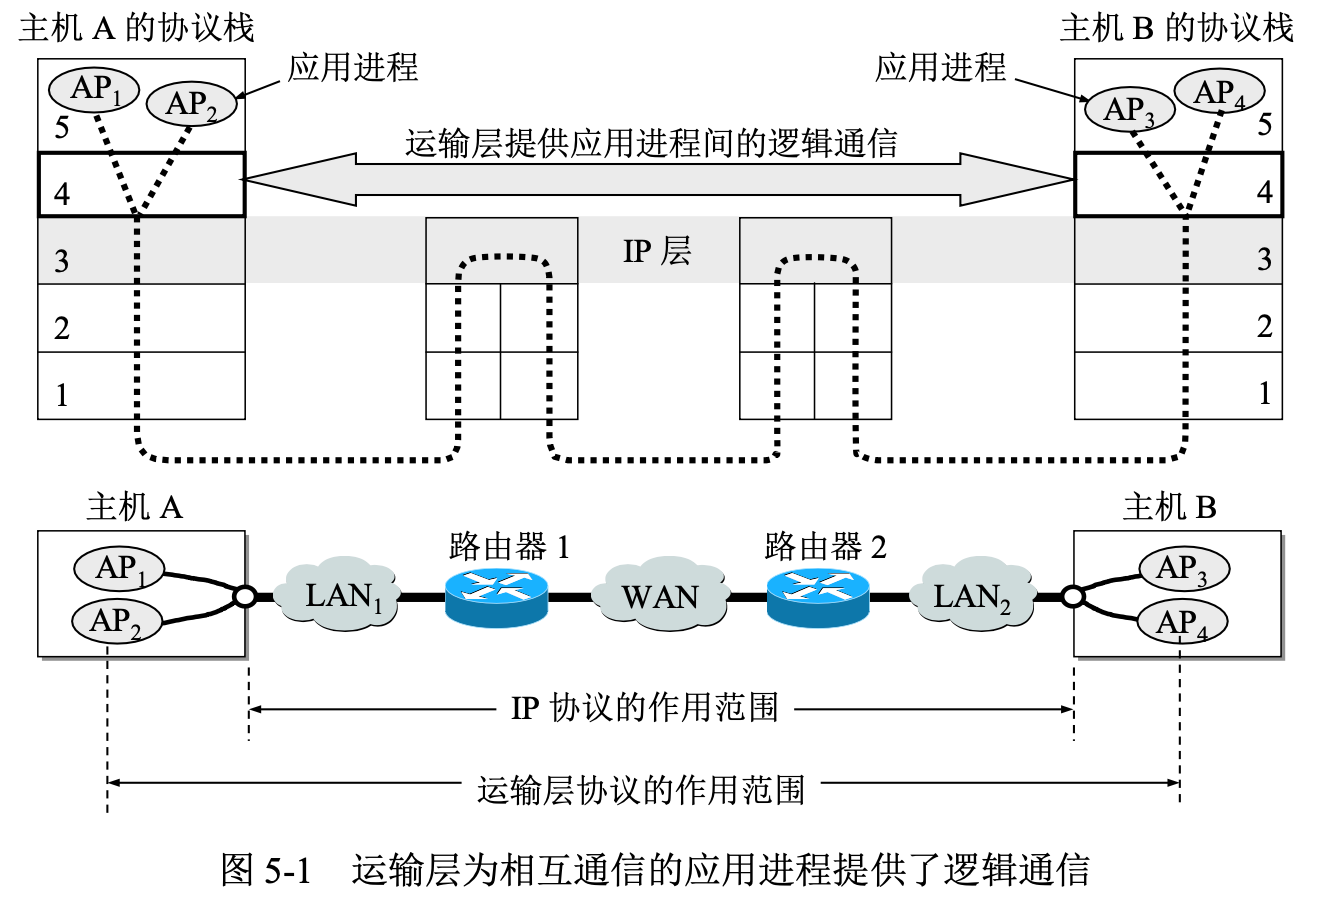
\includegraphics[width=0.7\textwidth]{img/5.1}
	\end{figure}

	\begin{itemize}
		\item 运输层有一个很重要的功能——复用(multiplexing)和分用(demultiplexing)
		\begin{itemize}
			\item “复用”是指在发送方不同的应用进程都可以使用同一个运输层协议传送数据
			\item “分用”是指接收方的运输层在剥去报文的首部后能够把这些数据正确交付目的应用进程
		\end{itemize}
		\item 运输层向高层用户屏蔽了下面网络核心的细节,它使应用进程看见的就是好像在两个运输层实体之间有一条端到端的逻辑通信信道
	\end{itemize}
	
	\begin{figure}[H]
		\centering
		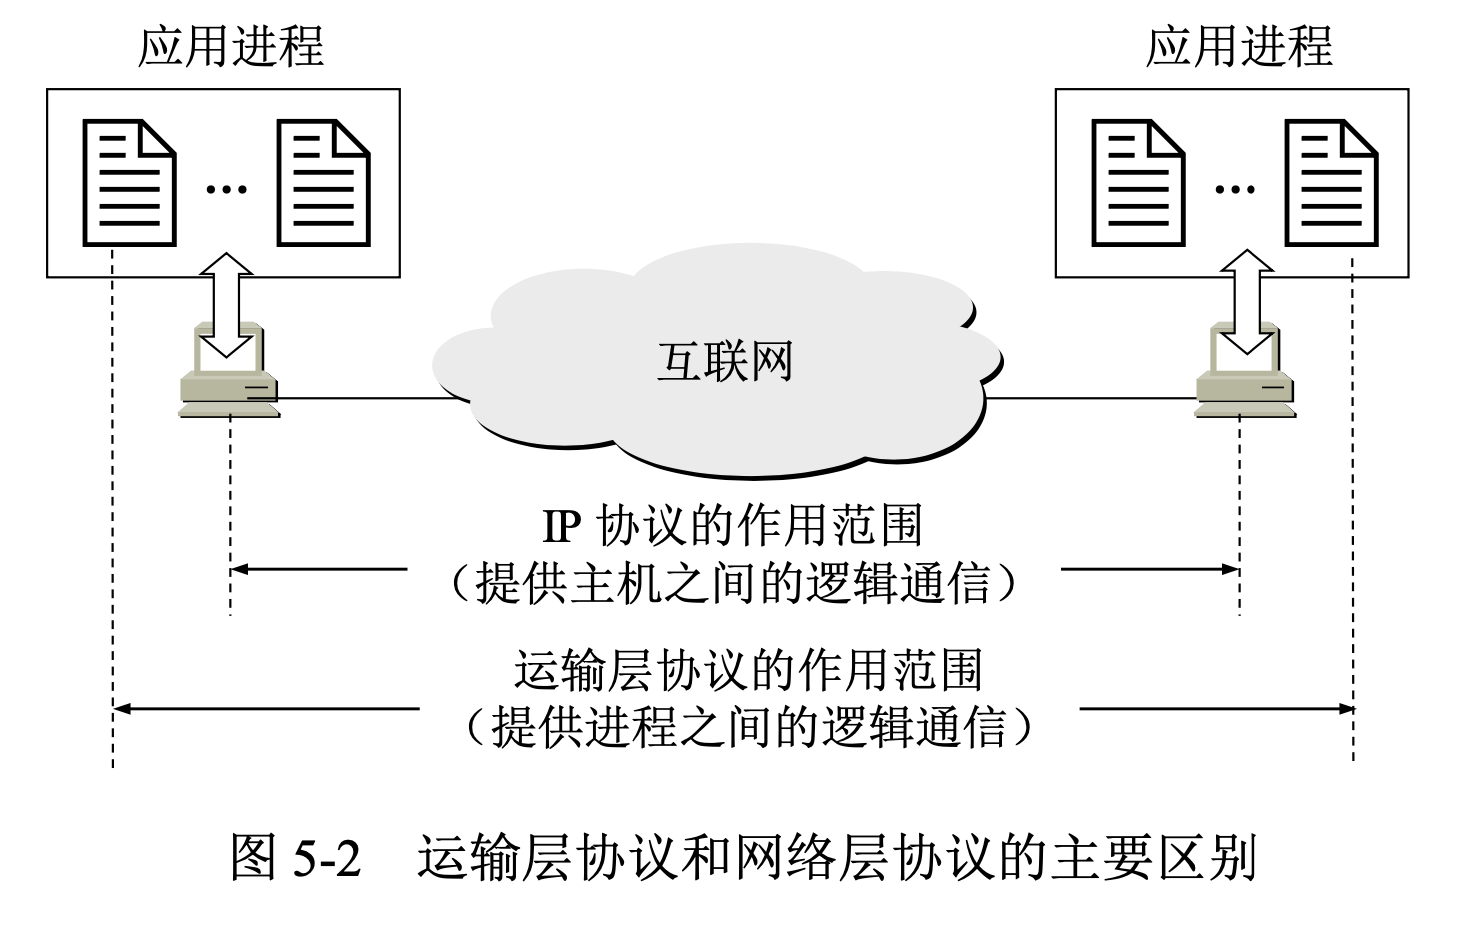
\includegraphics[width=0.55\textwidth]{img/5.2}
	\end{figure}

	\subsection{运输层的两个主要协议}
	TCP/IP 运输层的两个主要协议都是互联网的正式标准,即
	\begin{itemize}
		\item 用户数据报协议 UDP(User Datagram Protocol)
		\begin{itemize}
			\item UDP 在传送数据之前不需要先建立连接
			\item 远地主机的运输层在收到 UDP 报文后,不需要给出任何确认
			\item 虽然 UDP 不提供可靠交付,但在某些情况下 UDP 却是一种最有效的工作方式
		\end{itemize}
		\item 传输控制协议 TCP(Transmission Control Protocol)
		\begin{itemize}
			\item TCP 则提供面向连接的服务,在传送数据之前必须先建立连接,数据传送结束后要释放连接
			\item TCP 不提供广播或多播服务
			\item 由于 TCP 要提供可靠的、面向连接的运输服务,因此不可避免地增加了许多的开销,如确认、流量控制、计时器以及连接管理等。这不仅使协议数据单元的首部增大很多,还要占用许多的处理机资源
		\end{itemize}
	\end{itemize}

	\begin{figure}[H]
		\centering
		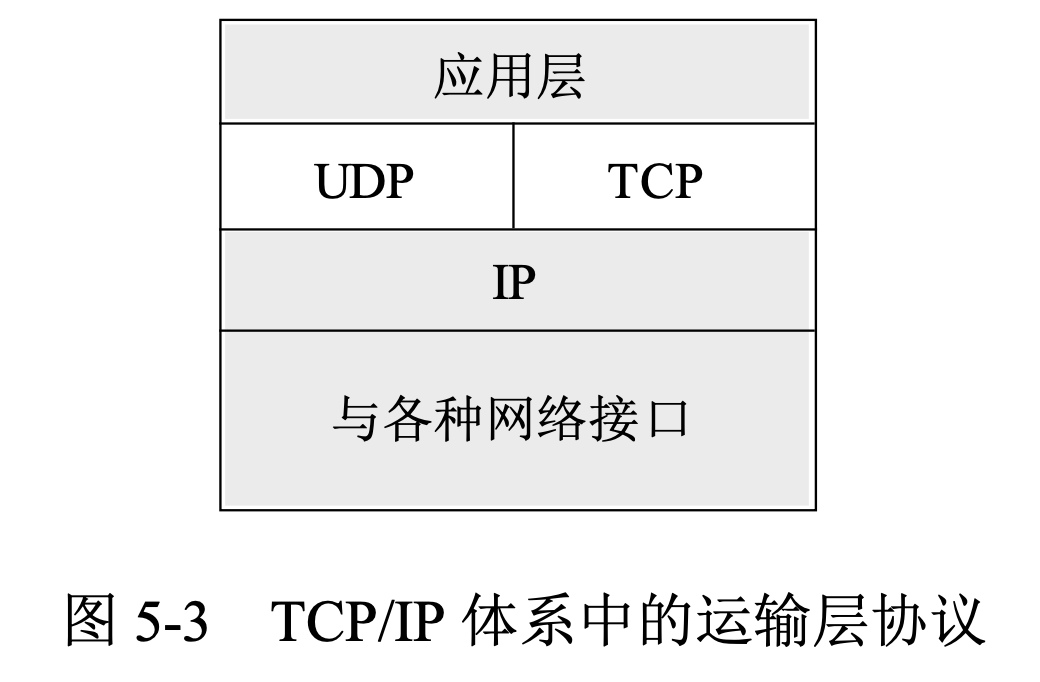
\includegraphics[width=0.3\textwidth]{img/5.3}
	\end{figure}

	使用 UDP 和 TCP 协议的各种应用和应用层协议
	\begin{table}[H]
		\centering
		\begin{tabular}{|c|c|c|}
		\hline
		应用      & 应用层协议          & 运输层协议 \\ \hline
		名字转换    & DNS(域名系统)      & UDP   \\ \hline
		文件传送    & TFTP(简单文件传送协议) & UDP   \\ \hline
		路由选择协议  & RIP(路由信息协议)    & UDP   \\ \hline
		IP 地址配置 & DHCP(动态主机配置协议) & UDP   \\ \hline
		网络管理    & SNMP(简单网络管理协议) & UDP   \\ \hline
		远程文件服务器 & NFS(网络文件系统)    & UDP   \\ \hline
		IP 电话   & 专用协议           & UDP   \\ \hline
		流式多媒体通信 & 专用协议           & UDP   \\ \hline
		多播      & IGMP(网际组管理协议)  & UDP   \\ \hline
		电子邮件    & SMTP(简单邮件传送协议) & TCP   \\ \hline
		远程终端接入  & TELNET(远程终端协议) & TCP   \\ \hline
		万维网     & HTTP(超文本传送协议)  & TCP   \\ \hline
		文件传送    & FTP(文件传送协议)    & TCP   \\ \hline
		\end{tabular}
	\end{table}

	\subsection{运输层的端口}
	\begin{itemize}
		\item 在单个计算机中的进程是用进程标识符 PID 来标志的
		\item 因为在互联网上使用的计算机的操作系统种类很多,而不同的操作系统又使用不同格式的进程标识符
		\item 为了使运行不同操作系统的计算机的应用进程能够互 相通信,就必须用统一的方法对 TCP/IP 体系的应用进程进行标志
		\item TCP/IP 体系的运输层使用端口号来区分应用层的不同应用进程
		\begin{itemize}
			\item 端口号用16比特表示,取值范围为 $0 \sim 65535$
			\begin{itemize}
				\item 熟知端口号:数值为 $0\sim 1023$,IANA 把这些端口号指派给了 TCP/IP 体系中最重要的一些应用程序
				\item 登记端口号:数值为 $1024 \sim 49151$,为没有熟知端口号的应用程序使用,使用这类端口号必须在 IANA 按照规定的手续登记,以防止重复
				\item 短暂端口号:数值为 $49152 \sim 65535$,留给客户进程选择暂时使用。当服务器进程收到客户进程的报文时,就知道了客户进程所使用的端口号,因而可以把数据发送给客户进程。通信结束后,刚才已使用过的客户端口号就不复存在,这个端口号就可以供其他客户进程使用
			\end{itemize}
			\item 端口号只具有本地意义,即端口号只是为了标识本计算机应用层中的各进程,在因特网中,不同计算机中的相同端口号是没有联系的
		\end{itemize}
	\end{itemize}

	常用的熟知端口号:
	\begin{table}[H]
		\centering
		\begin{tabular}{|c|c|c|c|c|c|c|c|c|c|}
		\hline
		应用程序 & FTP & TELNET & SMTP & DNS & TFTP & HTTP & SNMP & SNMP(trap) & HTTPS \\ \hline
		端口号  & 21  & 23     & 25   & 53  & 69   & 80   & 161  & 162        & 443   \\ \hline
		\end{tabular}
	\end{table}

	\section{用户数据报协议UDP}

	\subsection{UDP概述}

	UDP 的主要特点是:
	\begin{itemize}
		\item UDP 是无连接的,即发送数据之前不需要建立连接,因此减少了开销和发送数据之前的时延
		\item UDP 使用尽最大努力交付,即不保证可靠交付,因此主机不需要维持复杂的连接状态表
		\item UDP 是面向报文的。发送方的 UDP 对应用程序交下来的报文,在添加首部后就向下交付 IP 层,这就是说,应用层交给 UDP 多长的报文,UDP 就照样发送,即一次发送一个报文
	\end{itemize}

	\begin{figure}[H]
		\centering
		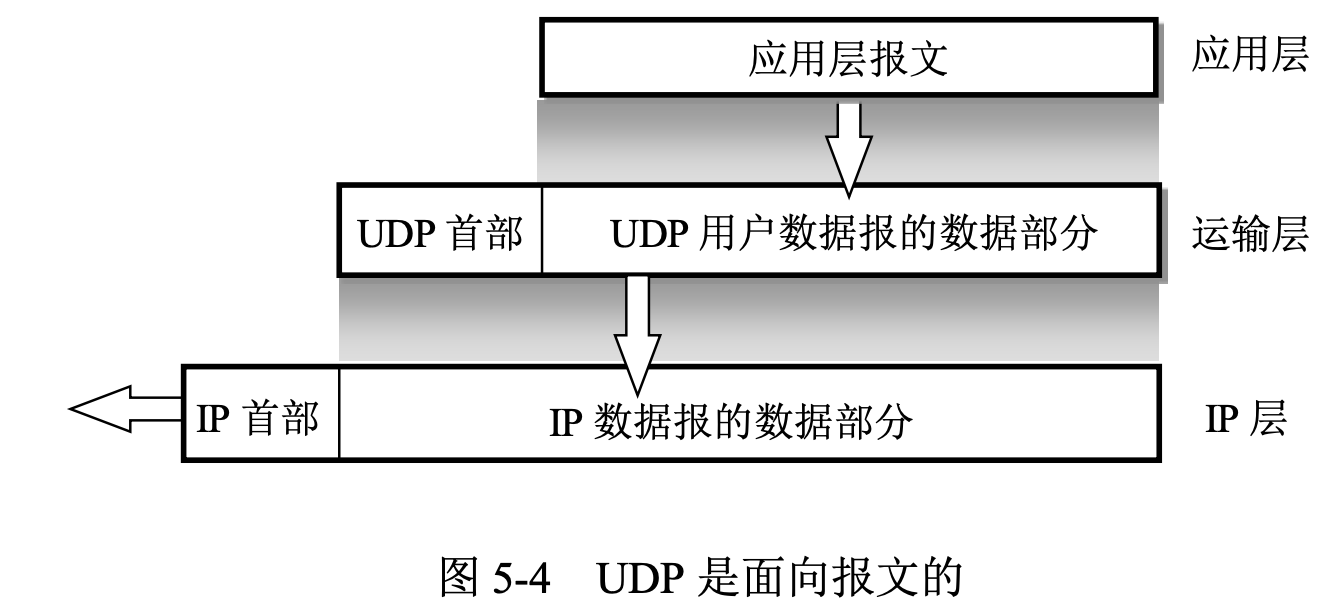
\includegraphics[width=0.45\textwidth]{img/5.4}
	\end{figure}

	\begin{itemize}
		\item UDP 没有拥塞控制,因此网络出现的拥塞不会使源主机的发送速率降低。这对某些实时应用是很重要的
		\item UDP 支持一对一、一对多、多对一和多对多的交互通信
		\item UDP 的首部开销小,只有 8 个字节,比 TCP 的 20 个字节的首部要短
	\end{itemize}

	\subsection{UDP的首部格式}
	用户数据报 UDP 有两个字段:数据字段和首部字段。首部字段很简单,只有 8 个字节,由四个字段组成,每个字段的长度都是两个字节。各字段意义如下:
	\begin{itemize}
		\item 源端口:源端口号。在需要对方回信时选用。不需要时可用全0
		\item 目的端口:目的端口号。这在终点交付报文时必须使用
		\item 长度:UDP用户数据报的长度,其最小值是8(仅有首部)
		\item 检验和:检测UDP用户数据报在传输中是否有错。有错就丢弃
	\end{itemize}

	\begin{figure}[H]
		\centering
		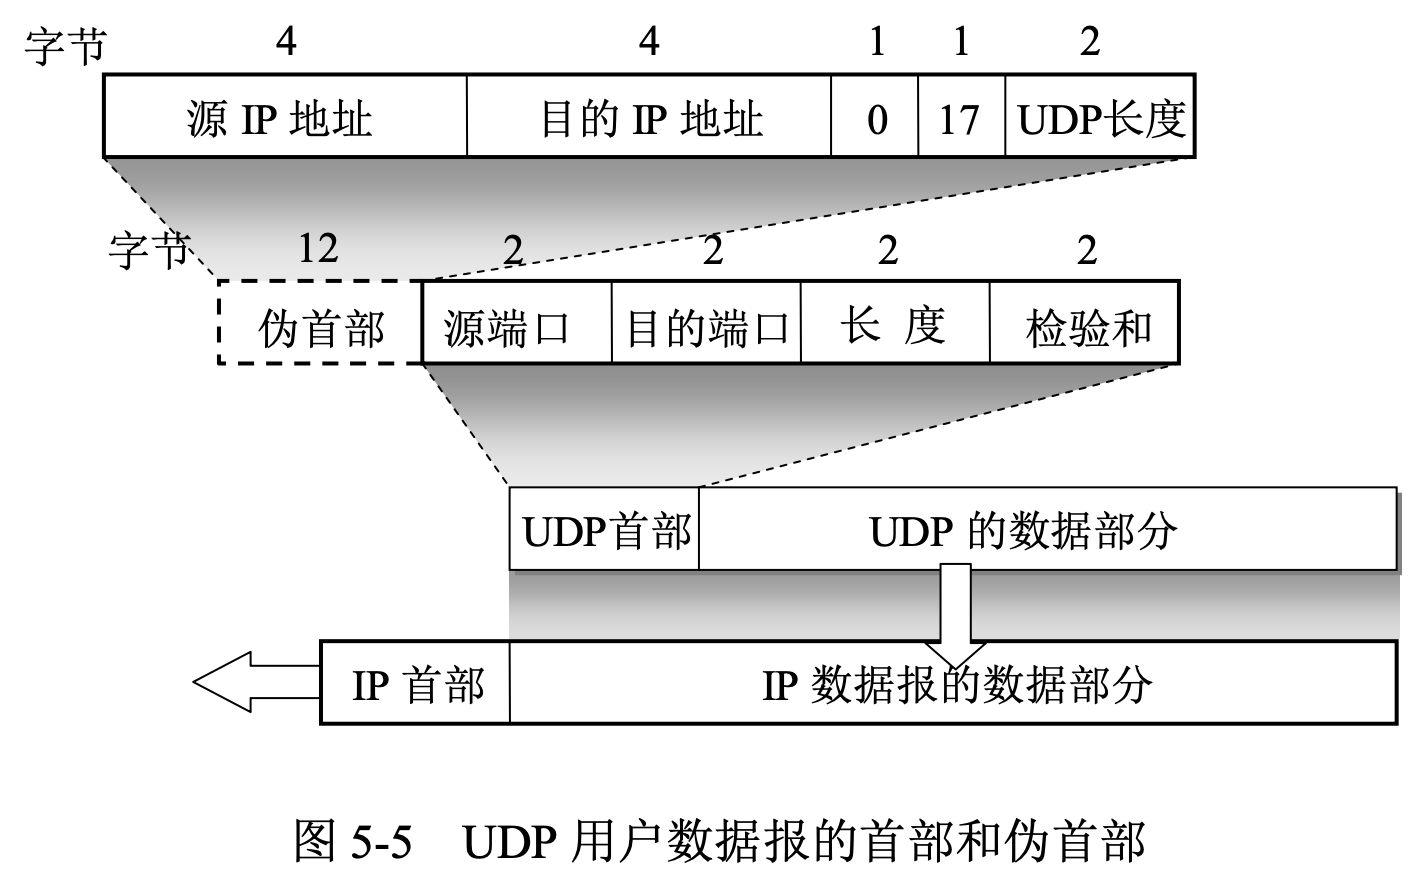
\includegraphics[width=0.65\textwidth]{img/5.5}
	\end{figure}

	UDP 用户数据报首部中检验和的计算方法
	\begin{itemize}
		\item 在计算检验和时,要在 UDP 用户数据报之前增加 12 个字节的伪首部
		\item 所谓“伪首部”是因为这种伪首部并不是 UDP 用户数据报真正的首部。只是在计算检验和时,临时添加在 UDP 用户数据报前面,得到一个临时的 UDP 用户数据报
		\item 检验和就是按照这个临时的 UDP 用户数据报来计算的
		\item 伪首部既不向下传送也不向上递交,而仅仅是为了计算检验和
		\item UDP 计算检验和的方法和计算 IP 数据报首部检验和的方法相似。但不同的是:IP 数据报的检验和只检验 IP 数据报的首部,但 UDP 的检验和是把首部和数据部分一起都检验
	\end{itemize}

	\section{传输控制协议TCP概述}

	\subsection{TCP最主要的特点}

	\begin{itemize}
		\item TCP 是面向连接的运输层协议。这就是说,应用程序在使用TCP协议之前,必须先建立 TCP 连接。在传送数据完毕后,必须释放已经建立的 TCP 连接
		\item 每一条 TCP 连接只能有两个端点(endpoint),每一条 TCP 连接只能是点对点的
		\item TCP 提供可靠交付的服务。通过 TCP 连接传送的数据,无差错、不丢失、不重复,并且按序到达
		\item TCP 提供全双工通信。TCP 允许通信双方的应用进程在任何时候都能发送数据。TCP 连接的两端都设有发送缓存和接收缓存,用来临时存放双向通信的数据
		\item 面向字节流。虽然应用程序和 TCP 的交互是一次一个数据块,但 TCP 把应用程序交下来的数据仅仅看成是一连串的无结构的字节流。TCP 并不知道所传送的字节流的含义。TCP 不保证接收方应用程序所收到的数据块和发送方应用程序所发出的数据块具有对应大小的关系。但接收方应用程序收到的字节流必须和发送方应用程序发出的字节流完全一样
	\end{itemize}

	\begin{figure}[H]
		\centering
		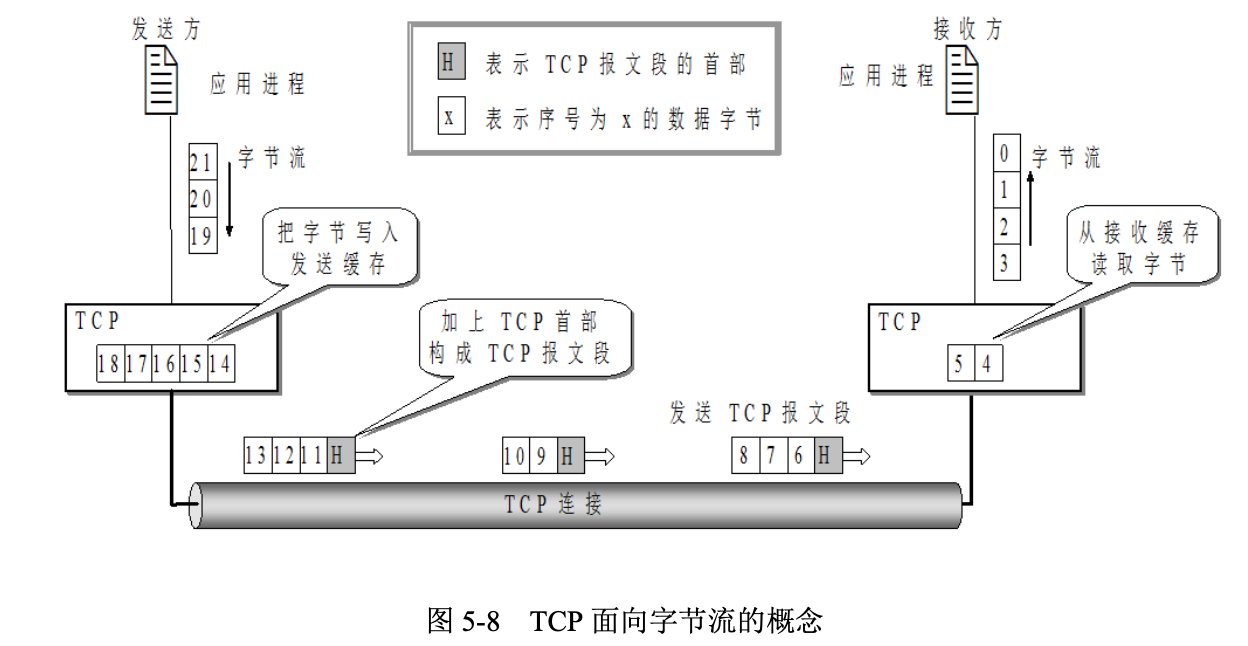
\includegraphics[width=0.65\textwidth]{img/5.8}
	\end{figure}

	\subsection{TCP的链接}
	\begin{itemize}
		\item TCP 把连接作为最基本的抽象
		\item TCP 连接的端点叫做套接字(socket)或插口。根据 RFC 793 的定义:端口号拼接到(concatenated with)IP 地址即构成了套接字,即
		$$\mbox{套接字}\  \mathrm{socket} =(\mathrm{IP} \mbox{地址}\ \mbox{:\ 端口号})$$
		\item 每一条 TCP 连接唯一地被通信两端的两个端点(即两个套接字)所确定。即:
		$$\mathrm{TCP} \mbox{连接} ::= \ \{\mathrm{socket_1,socket_2}\} = \{\mathrm{(IP_1:port_1),(IP_2:port_2)}\}$$
	\end{itemize}

	\section{TCP报文段的首部格式}
	TCP 报文段首部的前 20 个字节是固定的,后面有 $4n$ 字节是根据需要而增加的选项,因此 TCP 首部的最小长度是 20 字节
	\begin{figure}[H]
		\centering
		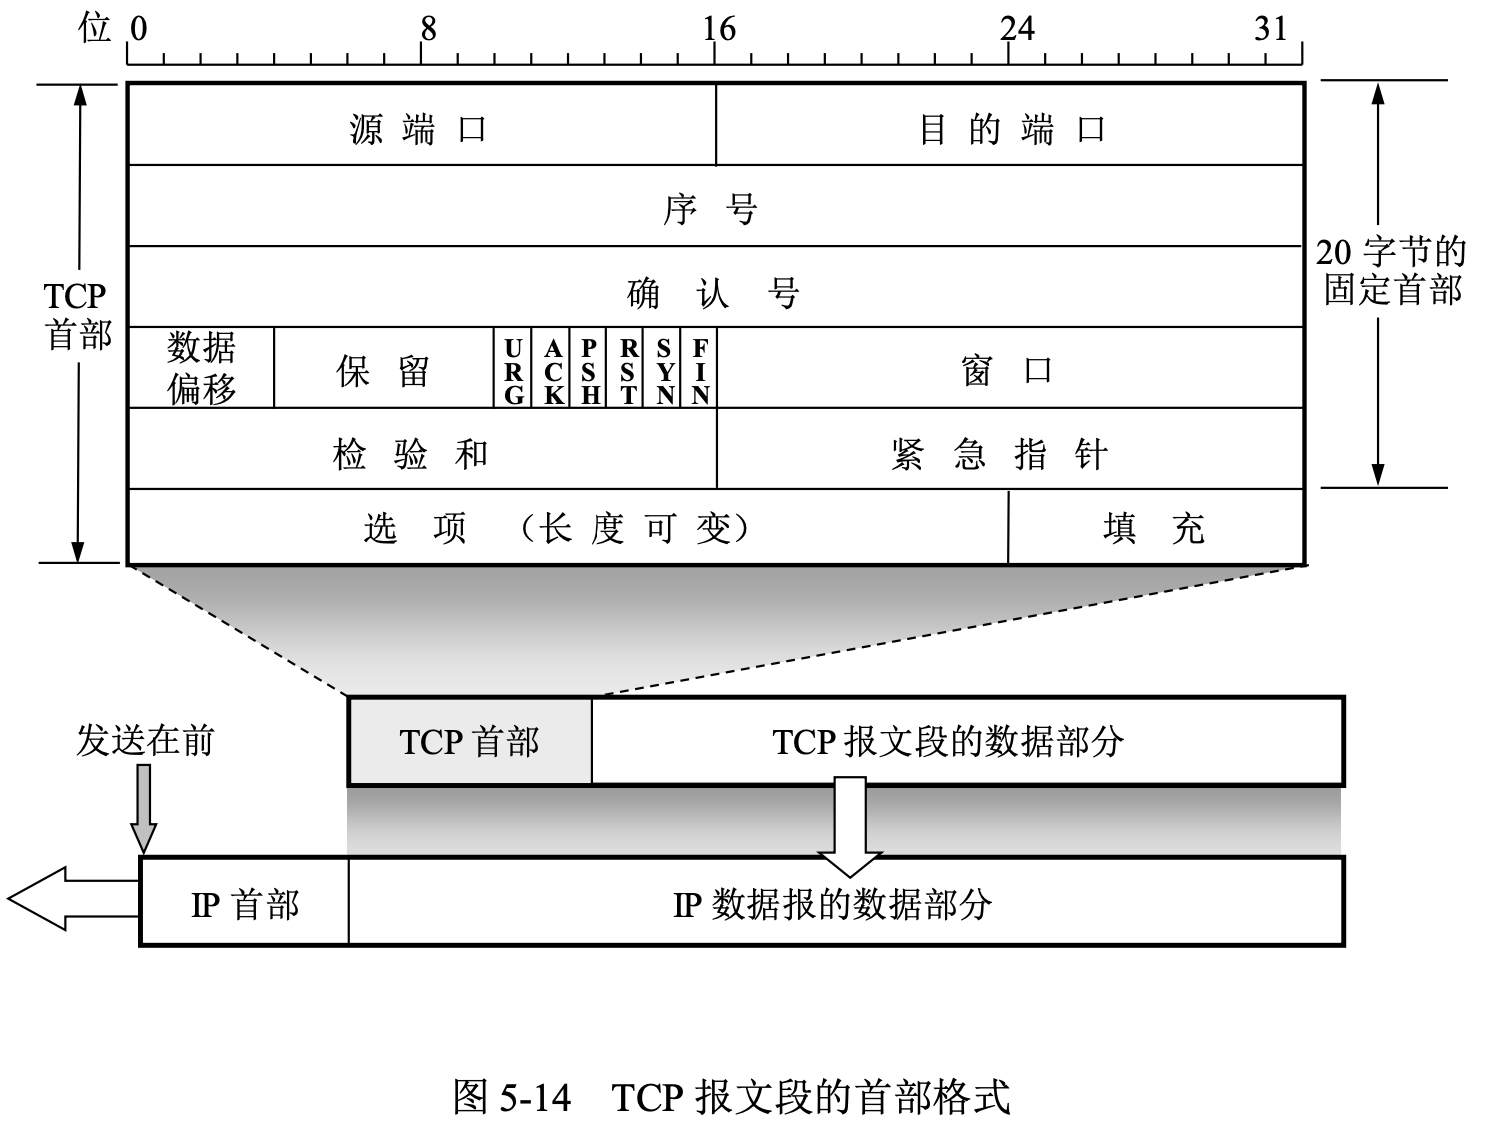
\includegraphics[width=0.6\textwidth]{img/5.14}
	\end{figure}

	首部固定部分各字段的意义如下:
	\begin{enumerate}[label=\arabic*.]
		\item 源端口和目的端口
		
		各占 2 字节(16 位),分别写入源端口号和目的端口号
		\item 序号
		\begin{itemize}
			\item 占 4 字节,取值范围是 $[0,2^{32} - 1]$,序号增加到 $2^{32}-1$ 后,下一个序号就又回到 0
			\item 用来指出本 TCP 报文段数据载荷的第一个字节的序号
		\end{itemize}
		\item 确认号
		\begin{itemize}
			\item 占 4 字节,取值范围是 $[0,2^{32} - 1]$,确认号增加到 $2^{32}-1$ 后,下一个确认号就又回到 0
			\item 用来指出期望收到对方下一个 TCP 报文段的数据载荷的第一个字节的序号,同时也是对之前收到的所有数据的确认
			\item 若确认号$=N$,则表明到序号 $N-1$ 为止的所有数据都已正确接收,期望接收序号为 $N$ 的数据
		\end{itemize}
		\item 数据偏移
		\begin{itemize}
			\item 占 4 位,并且以 4 字节为单位
			\item 用来指出 TCP 报文段的数据载荷部分的起始处距离 TCP 报文段的起始处有多远
			\item 这个字段实际上是指出了 TCP 报文段的首部长度
			\begin{itemize}
				\item 首部固定长度为 20 字节,因此数据偏移字段的最小值为 $(0101)_2$
				\item 首部最大长度为 60 字节,因此数据偏移字段的最大值为 $(1111)_2$
			\end{itemize}
		\end{itemize}
		\item 保留
		
		占 6 位,保留为今后使用,但目前应置为 0
		\item 紧急 URG(urgent)
		\begin{itemize}
			\item 当 URG = 1 时,表明紧急指针字段有效
			\item 它告诉系统此报文段中有紧急数据,应尽快传送,而不要按原来的排队顺序来传送
		\end{itemize}
		\item 确认 ACK(acknowledge)
		\begin{itemize}
			\item 仅当 ACK = 1 时确认号字段才有效;当 ACK = 0 时,确认号无效
			\item TCP 规定,在连接建立后所有传送的报文段都必须把 ACK 置 1
		\end{itemize}
		\item 推送 PSH(push)
		
		接收方 TCP 收到 PSH = 1 的报文段,就尽快地交付接收应用进程,而不再等到整个缓存都填满了后再向上交付
		\item 复位 RST(reset)
		\begin{itemize}
			\item 当 RST = 1 时,表明 TCP 连接中出现严重差错(如由于主机崩溃或其他原因),必须释放连接,然后再重新建立运输连接
			\item RST 置 1 还用来拒绝一个非法的报文段或拒绝打开一个连接
		\end{itemize}
		\item 同步 SYN(synchronization)
		
		在 TCP 连接建立时用来同步序号
		\item 终止 FIN(finish)
		
		用来释放 TCP 连接
		\item 窗口
		\begin{itemize}
			\item 占 2 字节,以字节为单位,指出发送本报文的一方的接受窗口
			\item 窗口值作为接收方让发送方设置其发送窗口的依据
			\item 这是以接收方的接收能力来控制发送方的发送能力,称为流量控制
		\end{itemize}
		\item 检验和
		\begin{itemize}
			\item 占 2 字节,检查范围包括 TCP 报文段的首部和数据载荷两部分
			\item 在计算检验和前,要在 TCP 报文段的首部加上 12 字节的伪首部
		\end{itemize}
		\item 紧急指针
		
		占 2 字节。紧急指针仅在 URG = 1 时才有意义,它指出本报文段中的紧急数据的字节数
		\item 选项
		
		长度可变,最长可达 40 字节
	\end{enumerate}

	\section{TCP可靠传输的实现}

	\subsection{以字节为单位的滑动窗口}

	假定现在 A 收到了 B 发来的确认报文段,其中窗口是 20 字节,确认号是 31,根据这两个数据,A 构造出自己的发送窗口如下
	\begin{figure}[H]
		\centering
		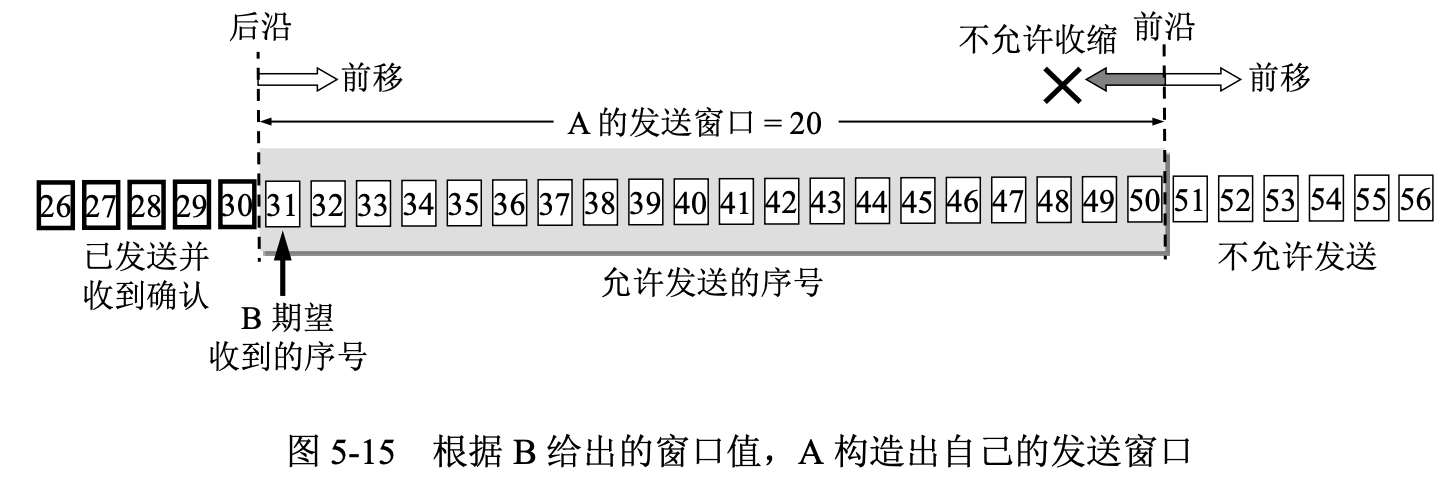
\includegraphics[width=0.85\textwidth]{img/5.15}
	\end{figure}

	发送窗口表示:在没有收到 B 的确认的情况下,A 可以连续把窗口内的数据都发送出去。凡是已经发送过的数据,在未收到确认之前都必须暂时保留,以便在超时重传时使用

	现在假定 A 发送了序号为 $31\sim 41$ 的数据。这时,发送窗口位置并未改变, 但发送窗口内靠后面有 11 个字节(灰色小方框表示)表示已发送但未收到确认。而发送窗口内靠前面的 9 个字节是允许发送但尚未发送的

	\begin{figure}[H]
		\centering
		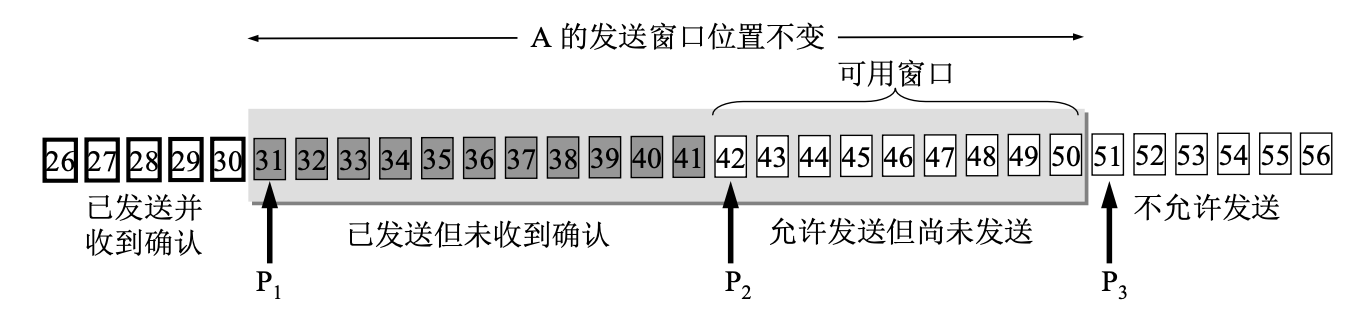
\includegraphics[width=0.85\textwidth]{img/5.16.1}
	\end{figure}

	假设 B 收到了序号为 32 和 33 的数据。这些数据没有按序到达,因为序号为 31 的数据没有收到(也许丢失了,也许滞留在网络中的某处),因此 B 向 A 发送确认号为 31 的确认报文段

	\begin{figure}[H]
		\centering
		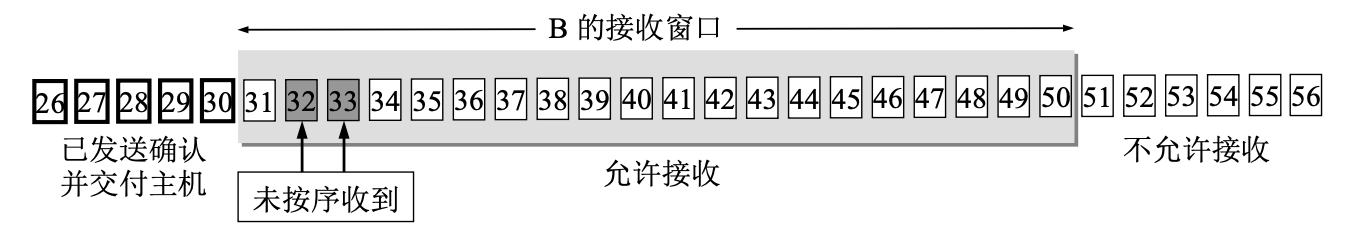
\includegraphics[width=0.85\textwidth]{img/5.16.2}
	\end{figure}

	现在假定 B 收到了序号为 31 的数据,并把序号为 $31\sim 33$ 的数据交付主机,然后 B 删除这些数据。接着把接收窗口向前移动 3 个序号,同时给 A 发送确认,其中窗口值仍为 20,但确认号是 34

	A 收到 B 的确认后,就可以把发送窗口向前滑动 3 个序号

	\begin{figure}[H]
		\centering
		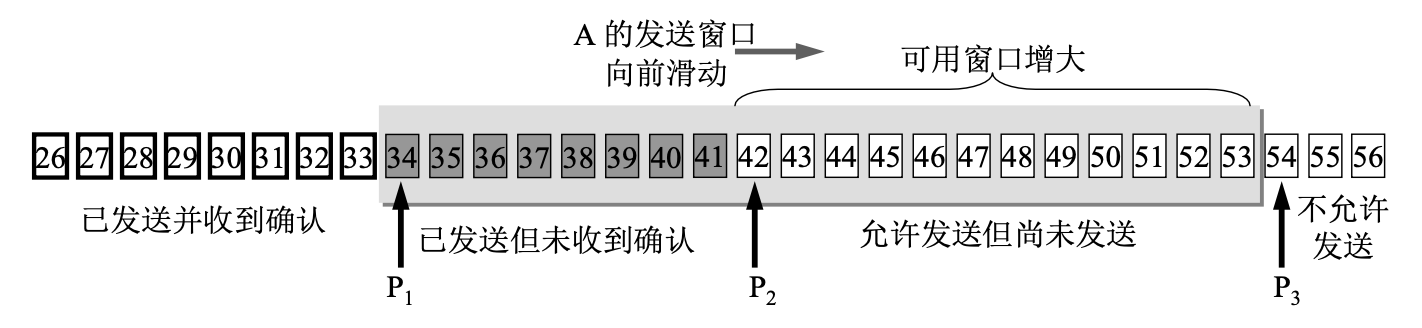
\includegraphics[width=0.85\textwidth]{img/5.17.1}
	\end{figure}

	A在继续发送完序号 $42\sim 53$ 的数据后,发送窗口内的序号都已用完,但还没有再收到确认,由于 A 的发送窗口已满,可用窗口已减小到零,因此必须停止发送

	\begin{figure}[H]
		\centering
		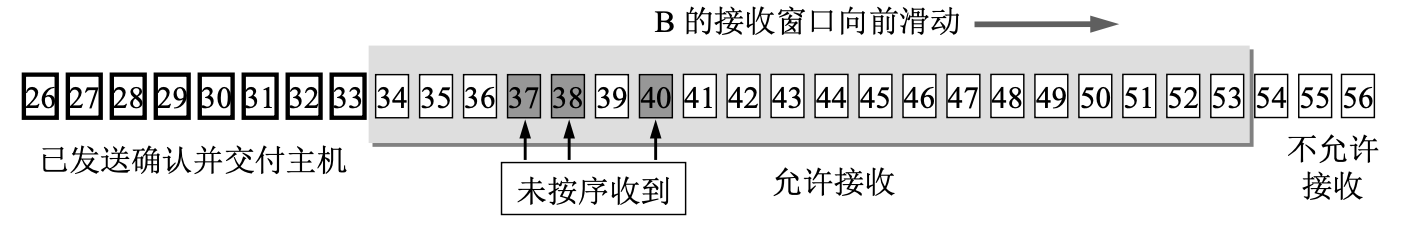
\includegraphics[width=0.85\textwidth]{img/5.17.2}
	\end{figure}

	A 在经过一段时间后(由超时计时器控制)重传这部分数据,重新设置超时计时器,直到收到 B 的确认为止。如果 A 收到确认号落在发送窗口内,那么 A 就可以使发送窗口继续向前滑动,并发送新的数据

	根据上面所讨论的例子,还有以下三点需要注意:
	\begin{itemize}
		\item 虽然 A 的发送窗口是根据 B 的接收窗口设置的,但在同一时刻,A 的发送窗口并不总是和 B 的接收窗口一样大
		\begin{itemize}
			\item 这是因为通过网络传送窗口值需要经历一定的时间滞后
			\item 另外发送方 A 还可能根据网络当时的拥塞情况适当减小自己的发送窗口数值
		\end{itemize}
		\item 对于不按序到达的数据应如何处理,TCP 标准并无明确规定
		\begin{itemize}
			\item 如果接收方把不按序到达的数据一律丢弃,那么接收窗口的管理将会比较简单,但这样做对网络资源的利用不利
			\item -因此 TCP 通常对不按序到达的数据是先临时存放在接收窗口中,等到字节流中所缺少的字节收到后,再按序交付上层的应用进程
		\end{itemize}
		\item TCP 要求接收方必须有累积确认的功能,这样可以减小传输开销。接收方可以在合适的时候发送确认,也可以在自己有数据要发送时把确认信息顺便捎带上
		\begin{itemize}
			\item 接收方不应过分推迟发送确认,否则会导致发送方不必要的重传,这反而浪费了网络的资源
			\begin{itemize}
				\item TCP 标准规定,确认推迟的时间不应超过 0.5 秒
				\item 若收到一连串具有最大长度的报文段,则必须每隔一个报文段就发送一个确认
			\end{itemize}
			\item 捎带确认实际上并不经常发生,因为大多数应用程序很少同时在两个方向上发送数据
		\end{itemize}
	\end{itemize}

	\subsection{超时重传时间的选择}
	\begin{itemize}
		\item TCP 采用了一种自适应算法,它记录一个报文段发出的时间,以及收到相应的确认的时间。这两个时间之差就是报文段的往返时间 RTT 
		\item TCP 保留了 RTT 的一个加权平均往返时间 $\mathrm{RTT_S}$
		\item 每当第一次测量到 RTT 样本时,$\mathrm{RTT_S}$ 值就取为所测量到的 RTT 样本值。但以后每测量到一个新的 RTT 样本,就按下式重新计算一次 $\mathrm{RTT_S}$:
		$$\mbox{新的}\,  \mathrm{RTT_S}  = (1-\alpha) \times (  \mbox{旧的}\,   \mathrm{RTT_S}) +\alpha \times (  \mbox{新的}\,   \mathrm{RTT}  \, \mbox{样本})$$
		\item RFC 6298 推荐 $\alpha$ 的取值为 0.125
		\item 显然,超时计时器设置的超时重传时间 RTO 应略大于上面得出的加权平均往返时间 $\mathrm{RTT_S}$。RFC 6298 建议使用下式计算 RTO:
		$$\mathrm{RTO = RTT_S + 4\times RTT_D}$$
		\item $\mathrm{RTT_D}$ 是 RTT 的偏差的加权平均值,它与 $\mathrm{RTT_S}$ 和新的 RTT 样本之差有关。RFC 6298 建议计算 $\mathrm{RTT_D}$:当第一次测量时,$\mathrm{RTT_D}$ 值取为测量到的 RTT 样本值的一半,在以后的测量中,则使用下式计算加权平均的 $\mathrm{RTT_D}$(其中 $\beta$ 的建议取值为 0.25):
		$$\mbox{新的}\,   \mathrm{RTT_D} = (1-\beta) \times ( \mbox{旧的}\,   \mathrm{RTT_D} ) + \beta \times |\mathrm{RTT_S} -  \mbox{新的}\,  \mathrm{RTT}\,  \mbox{样本} |$$
	\end{itemize}

	对于上面的算法若发生超时重传则会出现问题,如何判定此确认报文段是对先发送的报文段的确认,还是对后来重传的报文段的确认?

	\begin{figure}[H]
		\centering
		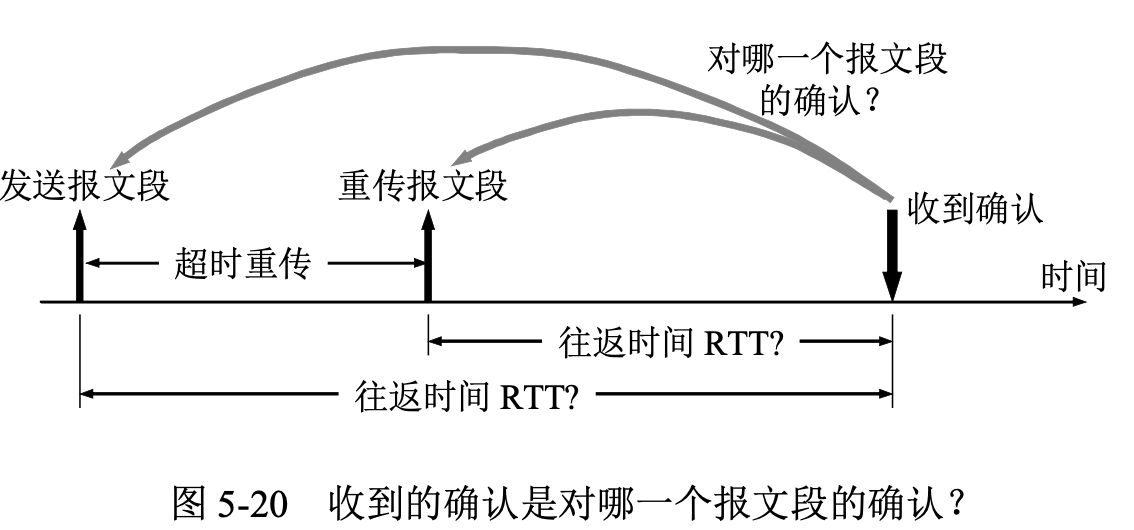
\includegraphics[width=0.6\textwidth]{img/5.20}
	\end{figure}

	\begin{itemize}
		\item 若收到的确认是对重传报文段的确认,但却被源主机当成是对原来的报文段的确认, 则这样计算出的 $\mathrm{RTT_S}$ 和超时重传时间 RTO 就会偏大
		\item 若收到的确认是对原来的报文段的确认,但被当成是对重传报文段的确认,则 由此计算出的 $\mathrm{RTT_S}$和 RTO 都会偏小
	\end{itemize}

	对此,Karn 提出了一个算法:在计算加权平均 $\mathrm{RTT_S}$ 时,只要报文段重传了,就不采用其往返时间样本。这样得出的加权平均 $\mathrm{RTT_S}$ 和 RTO 就较准确

	但是,这又引起新的问题。设想出现这样的情况:报文段的时延突然增大了很多。因此在原来得出的重传时间内,不会收到确认报文段。于是就重传报文段。但根据 Karn 算法,不考虑重传的报文段的往返时间样本。这样,超时重传时间就无法更新

	因此要对 Karn 算法进行修正。方法是:报文段每重传一次,就把超时重传时间 RTO 增大一些。典型的做法是取新的重传时间为旧的重传时间的 2 倍。当不再发生报文段的重传时,才根据上面的式子计算超时重传时间

	\section{TCP的流量控制}
	流量控制(flow control)就是让发送方的发送速率不要太快,要让接收方来得及接收

	下图中起始时 B 的接收窗口为 400 字节,图中未直接画出
	\begin{figure}[H]
		\centering
		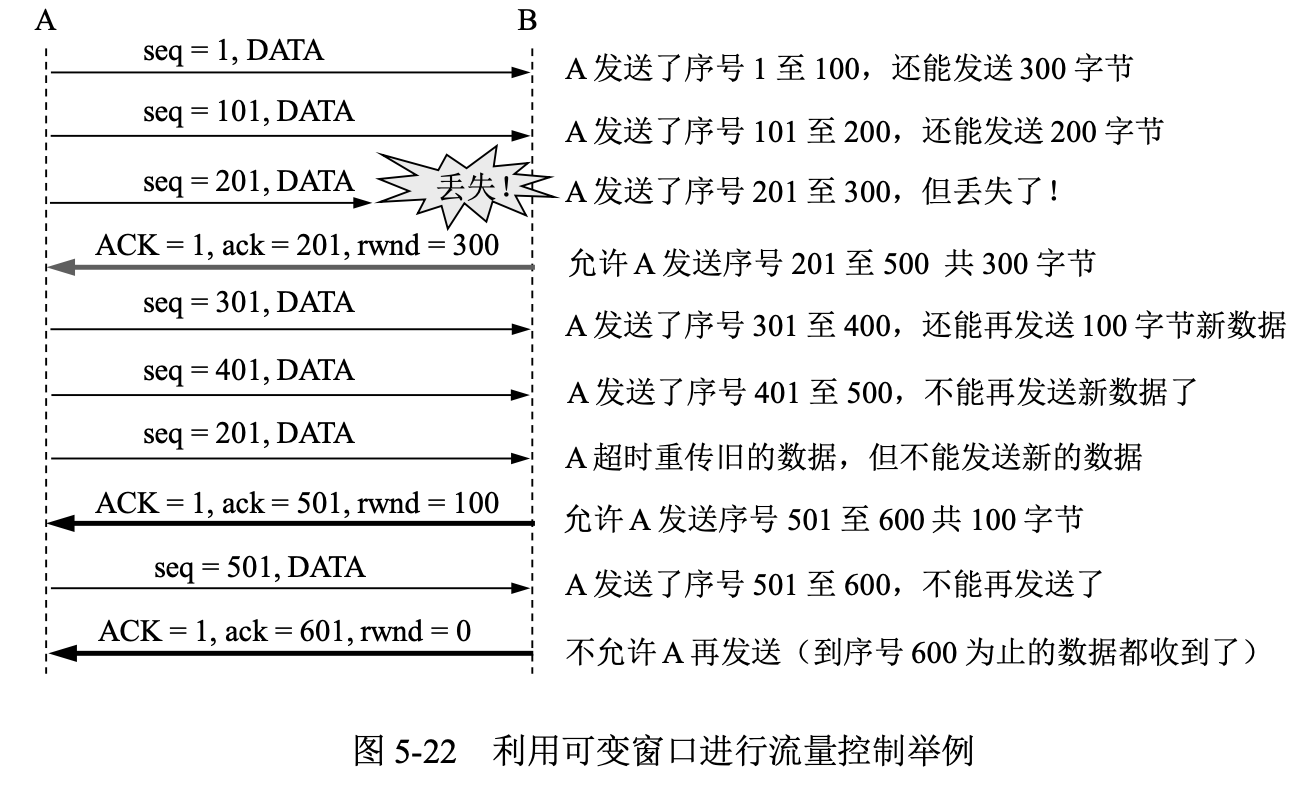
\includegraphics[width=0.7\textwidth]{img/5.22}
	\end{figure}

	现在考虑这样一种情况,上图中 B 向 A 发送了零窗口的报文段后不久,B 的接收缓存又有了一些存储空间。于是 B 向 A 发送了 rwnd = 400 的报文段。然而这个报文段在传送过程中丢失了。A 一直等待收到 B 发送的非零窗口的通知,而 B 也一直等待 A 发送的数据。如果没有其他措施,这种互相等待的死锁局面将一直延续下去。

	为了解决这个问题,TCP 为每一个连接设有一个持续计时器(persistence timer)。只要 TCP 连接的一方收到对方的零窗口通知,就启动持续计时器。若持续计时器设置的时间到期,就发送一个零窗口探测报文段(仅携带 1 字节的数据),而对方就在确认这个探测报文段时给出了现在的窗口值。如果窗口仍然是零,那么收到这个报文段的一方就重新设置持续计时器。如果窗口不是零,那么死锁的僵局就可以打破了。

	\section{TCP的拥塞控制}

	\begin{itemize}
		\item 在某段时间,若对网络中某一资源的需求超过了该资源所能提供的可用部分,网络的性能就要变坏。这种情况就叫做拥塞(congestion)
		\item 若出现拥塞而不进行控制,整个网络的吞吐量将随输入负荷的增大而下降
	\end{itemize}

	\begin{figure}[H]
		\centering
		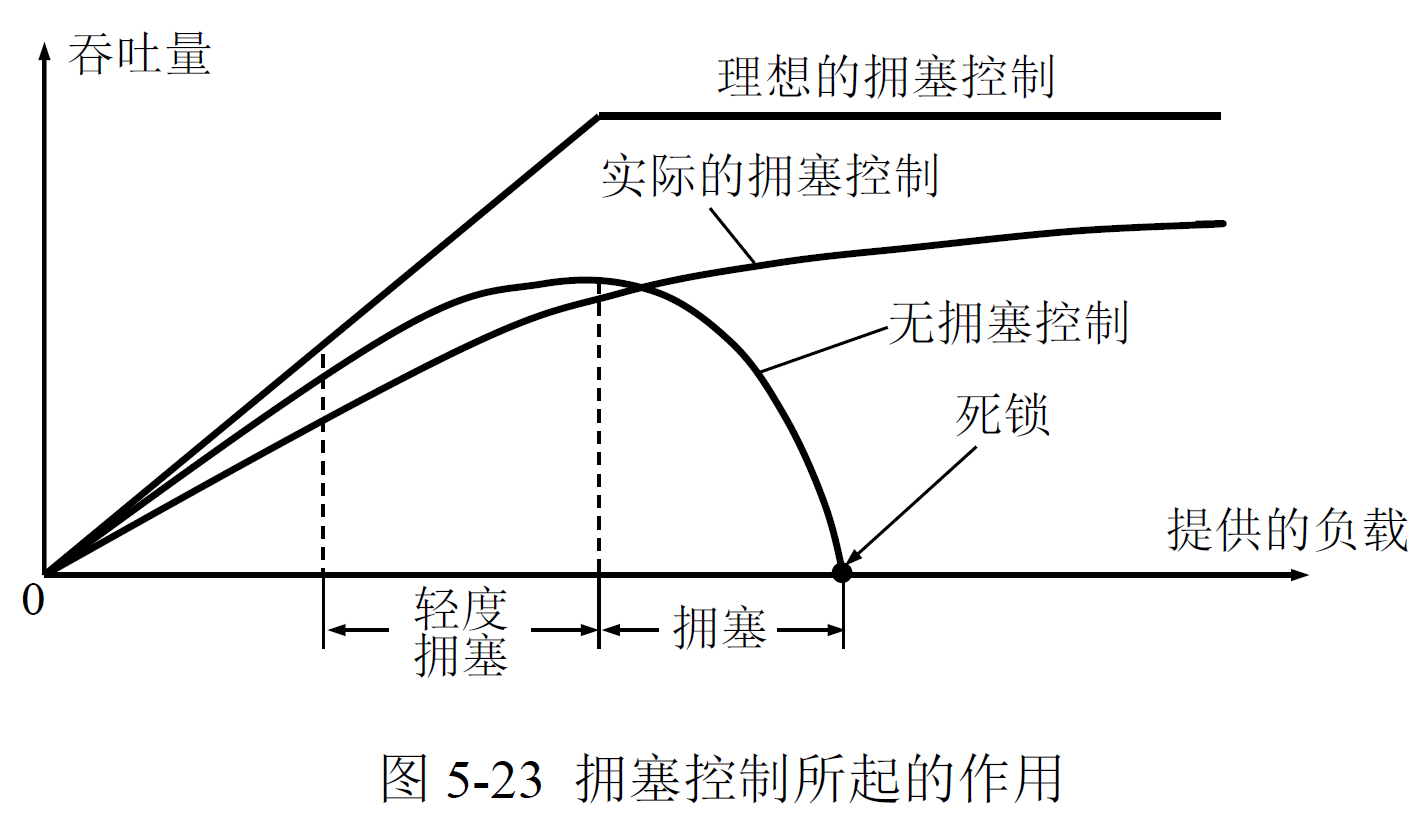
\includegraphics[width=0.6\textwidth]{img/5.23}
	\end{figure}

	TCP 进行拥塞控制的算法有四种, 即慢开始(slow-start) 、拥塞避免(congestion
	avoidance)、快重传(fast retransmit)和快恢复(fast recovery)

	为了集中精力讨论拥塞控制,下面假定:
	\begin{enumerate}[label=\arabic*.]
		\item 数据是单方向传送的,对方只传送确认报文
		\item 接收方总是有足够大的缓存空间,因而发送窗口的大小由网络的拥塞程度来决定
	\end{enumerate}

	\subsection{慢开始和拥塞避免}
	\begin{itemize}
		\item 发送方维护一个叫做拥塞窗口 cwnd 的状态变量,其值取决于网络的拥塞程度,并且动态变化
		\begin{itemize}
			\item 拥塞窗口 cwnd 的维护原则:只要网络没有出现拥塞,拥塞窗口就再增大一些;但只要网络出现拥塞,拥塞窗口就减小一些
			\item 判断发生网络拥塞的依据:没有按时收到应当到达的确认报文(即发生超时重传)
		\end{itemize}
		\item 发送方将拥塞窗口作为发送窗口 swnd,即 swnd = cwnd
		\item 维护一个慢开始门限 ssthresh 状态变量:
		\begin{itemize}
			\item 当 cwnd < ssthresh 时,使用慢开始算法
			\item 当 cwnd > ssthresh 时,停止使用慢开始算法,而改用拥塞避免算法
			\item 当 cwnd = ssthresh 时,既可以使用慢开始算法,也可以使用拥塞避免算法
		\end{itemize}
	\end{itemize}

	慢开始算法的思路是:当主机开始发送数据时,由于并不清楚网络的负荷情况,较好的方法是先探测一下,即由小到大逐渐增大发送窗口,也就是说,由小到大逐渐增大拥塞窗口数值

	慢开始规定,在每收到一个对新报文段的确认后,可以把拥塞窗口增加最多一个 SMSS(发送方最大报文段)的数值,如下面例子所示
	\footnote{下图中以报文段的个数作为窗口大小的单位,以传输轮次作为时间单位。一个传输轮次所经历的时间是往返时间 RTT,使用“传输轮次”是为了强调把拥塞窗口 cwnd 所允许发送的报文段都连续发送出去,并收到了对已发送的最后一个字节的确认}

	\begin{figure}[H]
		\centering
		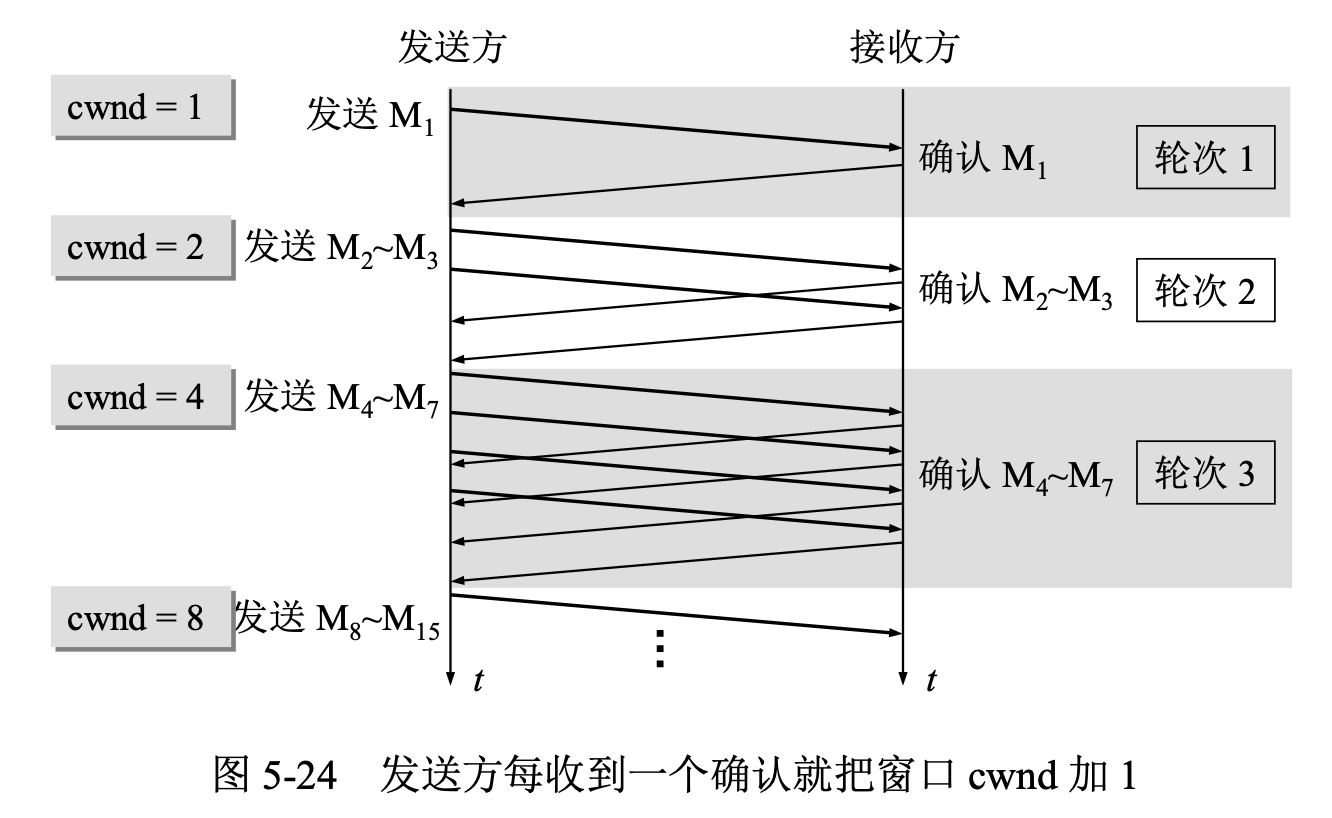
\includegraphics[width=0.8\textwidth]{img/5.24}
	\end{figure}

	拥塞避免算法的思路是让拥塞窗口 cwnd 缓慢增大,即每经过一个往返时间 RTT 就把发送方的拥塞窗口 cwnd 加1,而不是像慢开始阶段那样加倍增长

	\begin{figure}[H]
		\centering
		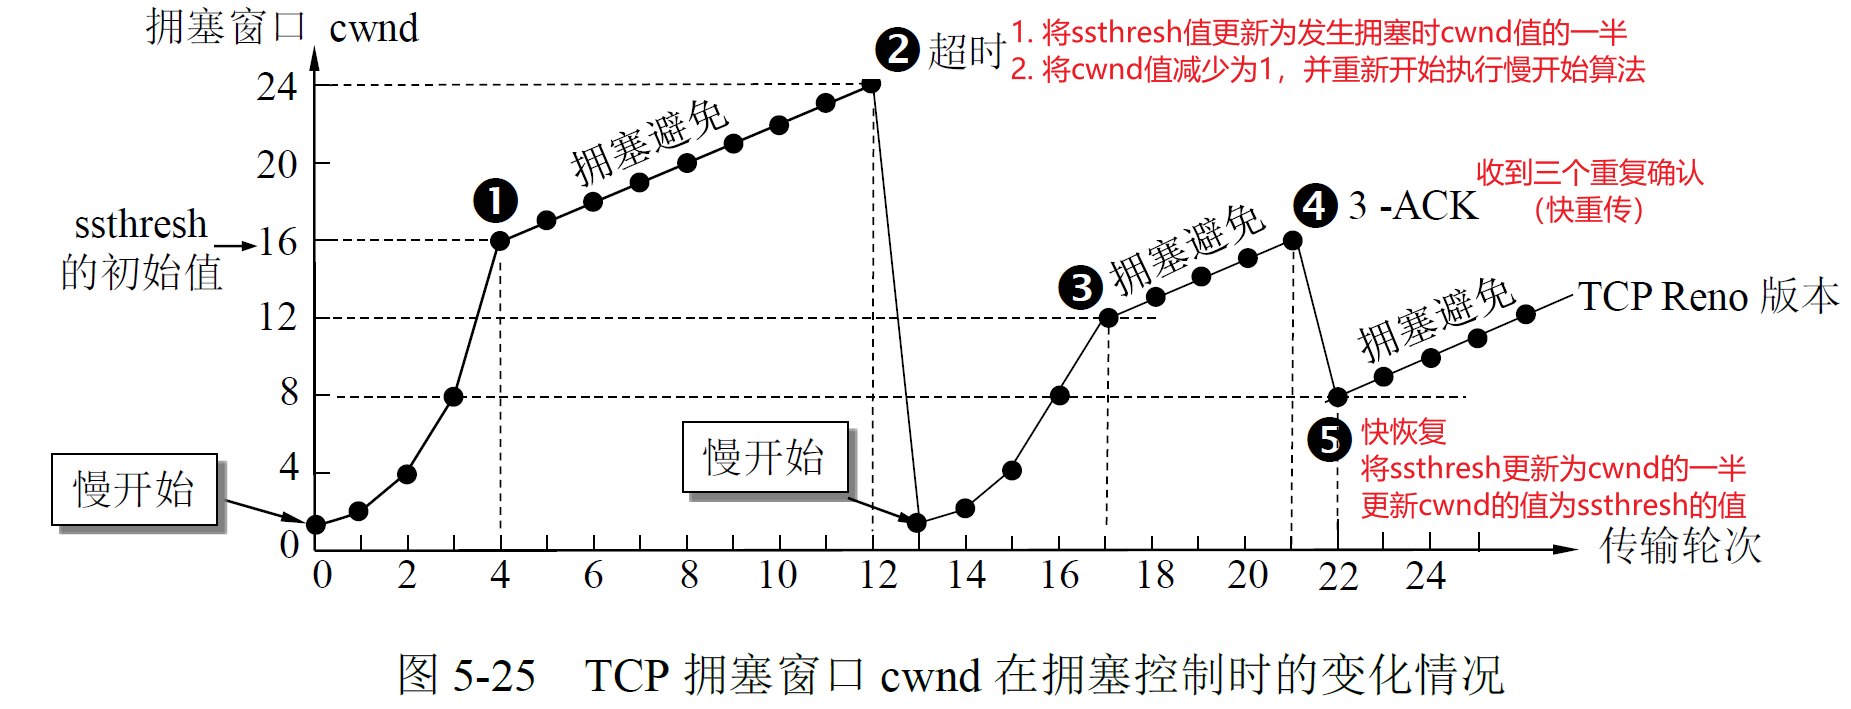
\includegraphics[width=0.9\textwidth]{img/5.25}
	\end{figure}

	\subsection{快重传和快恢复}
	\begin{itemize}
		\item 慢开始和拥塞避免算法是 1988 年提出的 TCP 拥塞控制算法(TCP Tahoe 版本)
		\item 1990 年又增加了两个新的拥塞控制算法(改进 TCP 的性能),这就是快重传和快恢复(TCP Reno 版本)
		\begin{itemize}
			\item 有时,个别报文段会在网络中丢失,但实际上网络并未发生拥塞
			\begin{itemize}
				\item 这将导致发送方超时重传,并误认为网络发生了拥塞
				\item 发送方把拥塞窗口 cwnd 又设置为最小值 1,并错误地启动慢开始算法,因而降低了传输效率
			\end{itemize}
		\end{itemize}
		\item 采用快重传算法就可以让发送方尽早知道发生了个别报文段的丢失
	\end{itemize}

	所谓快重传,就是使发送方尽快进行重传,而不是等超时重传计时器超时再重传
	\begin{itemize}
		\item 要求接收方不要等待自己发送数据时才进行捎带确认,而是要立即发送确认
		\item 即使收到了失序的报文段也要立即发出对已收到的报文段的重复确认
		\item 发送方一旦收到 3 个连续的重复确认,就将相应的报文段立即重传,而不是等该报文段的超时重传计时器超时再重传
		\item 对于个别丢失的报文段,发送方不会出现超时重传,也就不会误认为出现了拥塞(进而降低拥塞窗口 cwnd 为1)。使用快重传可以使整个网络的吞吐量提高约 20\%
	\end{itemize}

	\begin{figure}[H]
		\centering
		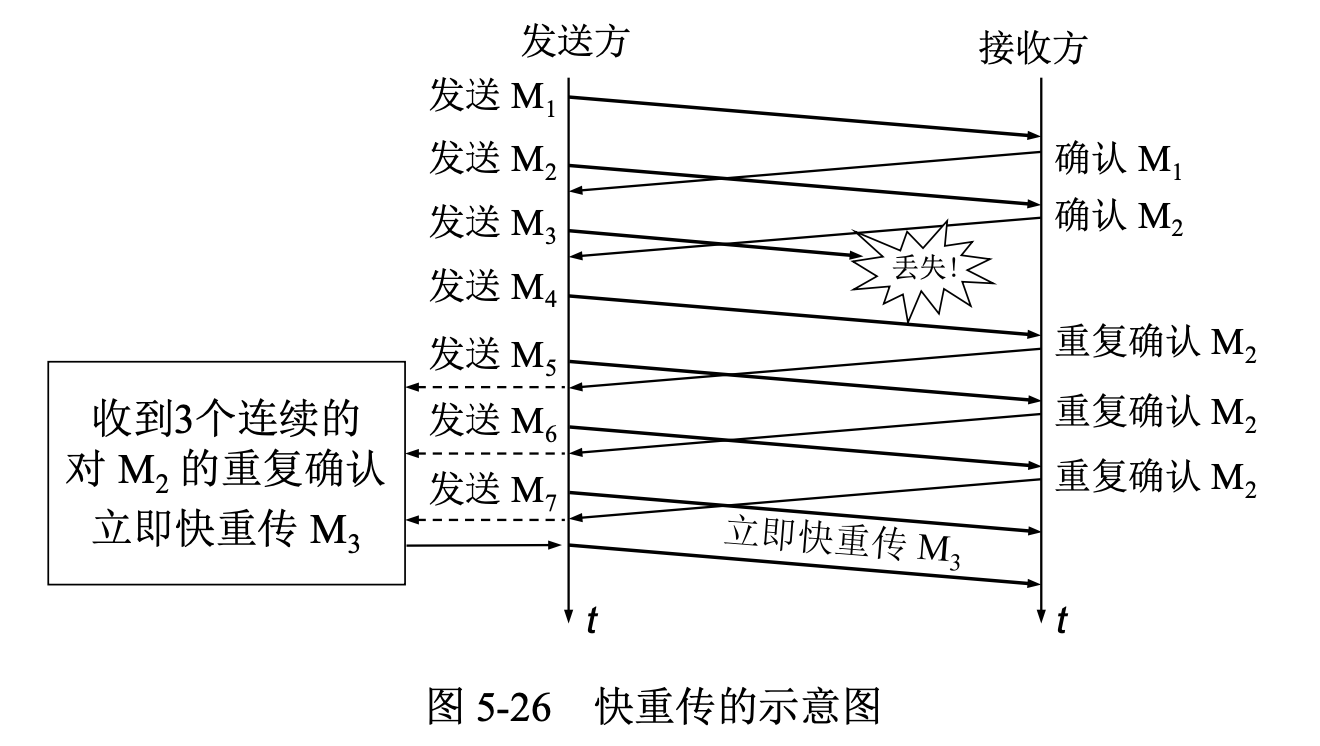
\includegraphics[width=0.7\textwidth]{img/5.26}
	\end{figure}

	发送方一旦收到 3 个重复确认,就知道现在只是丢失了个别的报文段。于是不启动慢开始算法,而执行快恢复算法
	\begin{itemize}
		\item 发送方将慢开始门限 ssthresh 值和拥塞窗口 cwnd 值调整为当前窗口的一半,开始执行拥塞避免算法
		\item 也有的快恢复实现是把快恢复开始时的拥塞窗口 cwnd 值再增大一些,即等于新的 ssthresh + 3
		\begin{itemize}
			\item 既然发送方收到 3 个重复的确认,就表明有 3 个数据报文段已经离开了网络
			\item 这 3 个报文段不再消耗网络资源而是停留在接收方的接收缓存中
			\item 可见现在网络中不是堆积了报文段而是减少了 3 个报文段,因此可以适当把拥塞窗口扩大些
		\end{itemize}
	\end{itemize}

	\section{TCP的运输连接管理}
	在 TCP 连接建立过程中要解决以下三个问题:
	\begin{enumerate}[label=\arabic*.]
		\item 要使每一方能够确知对方的存在
		\item 要允许双方协商一些参数(如最大窗口值、是否使用窗口扩大选项和时间戳选项以及服务质量等)
		\item 能够对运输实体资源(如缓存大小、连接表中的项目等)进行分配
	\end{enumerate}

	TCP 连接的建立采用客户服务器方式。主动发起连接建立的应用进程叫做客户(client),而被动等待连接建立的应用进程叫做服务器(server)

	\subsection{TCP的连接建立}
	\begin{figure}[H]
		\centering
		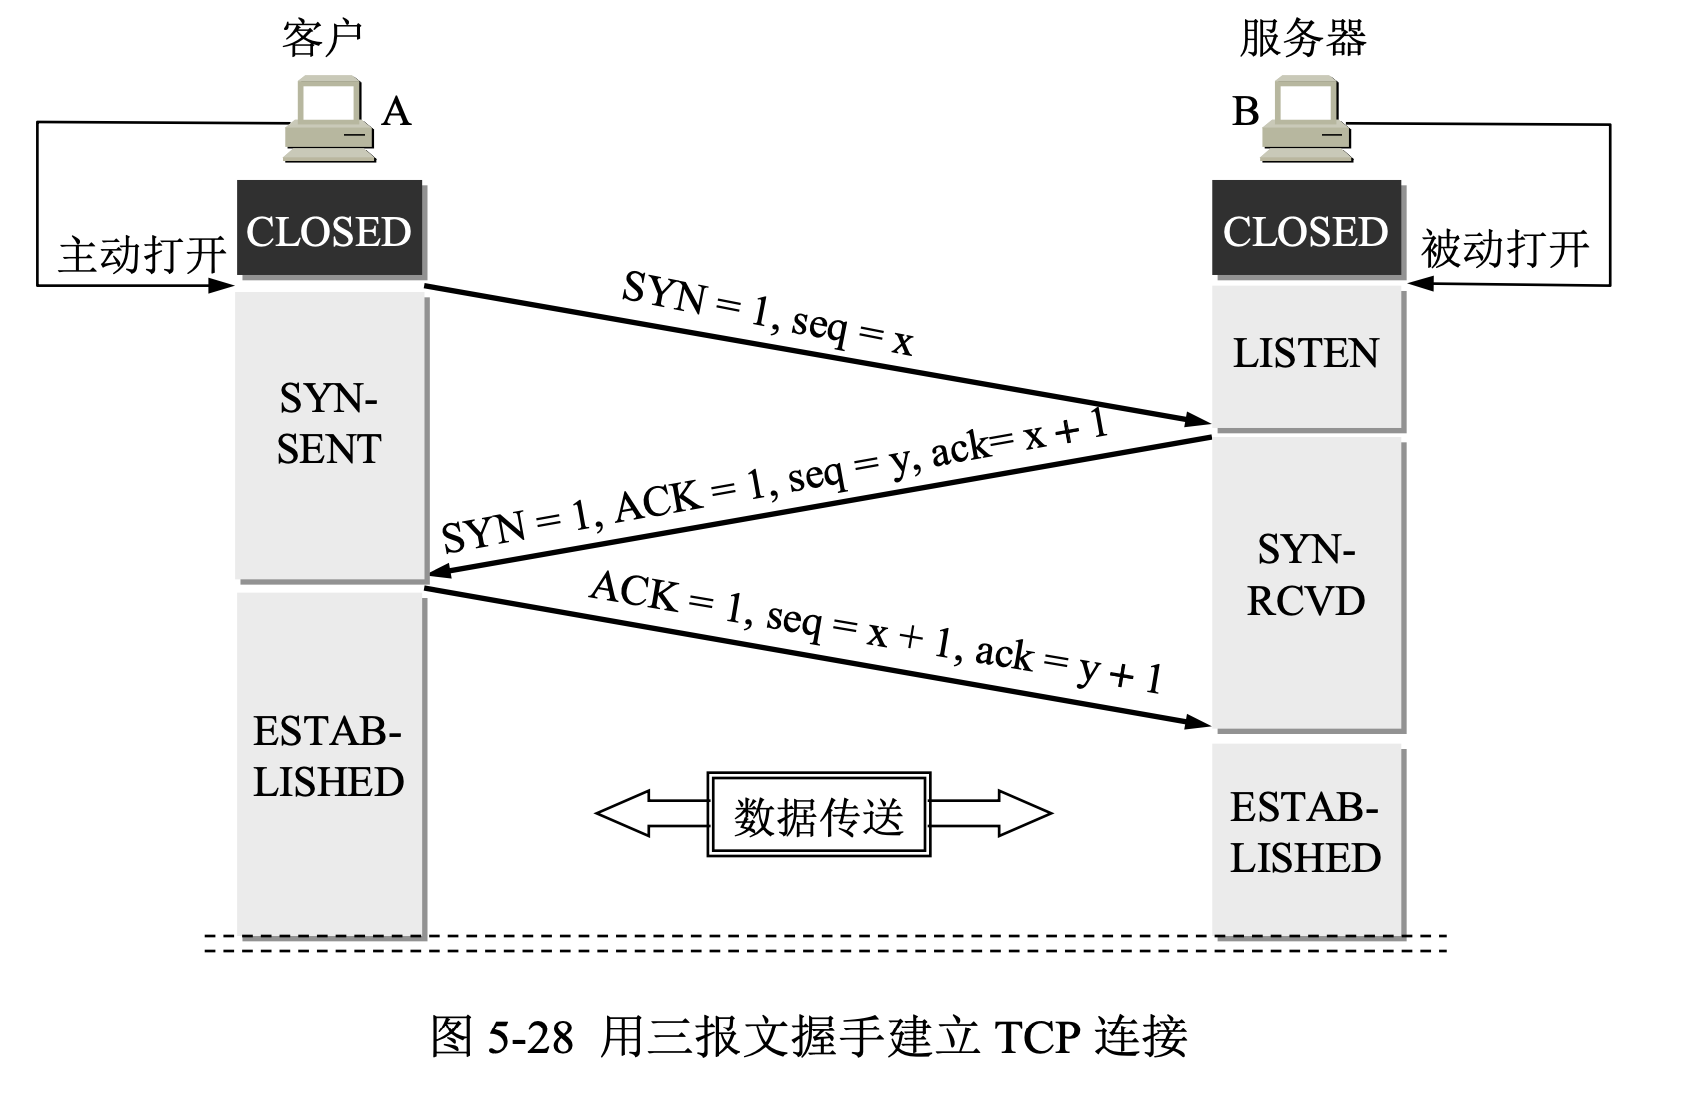
\includegraphics[width=0.65\textwidth]{img/5.28}
	\end{figure}

	开始时,B 的 TCP 服务器进程先创建传输控制块 TCB,准备接受客户进程的连接请求。然后服务器进程就处于 LISTEN(收听)状态,等待客户的连接请求。如有,即作出响应。

	A 的 TCP 客户进程也是首先创建传输控制模块 TCB。然后,在打算建立 TCP 连接时,向 B 发出连接请求报文段,这时首部中的同步位 SYN = 1,同时选择一个初始序号 seq = $x$。TCP 规定,SYN 报文段(即 SYN = 1 的报文段)不能携带数据,但要消耗掉一个序号。这时,TCP 客户进程进入 SYN-SENT(同步已发送)状态

	B 收到连接请求报文段后,如同意建立连接,则向 A 发送确认。在确认报文段中应把 SYN 位和 ACK 位都置 1,确认号是 ack = $x + 1$,同时也为自己选择一个初始序号 seq = $y$。请注意,这个报文段也不能携带数据,但同样要消耗掉一个序号。这时 TCP 服务器进程进入 SYN-RCVD(同步收到)状态

	TCP 客户进程收到 B 的确认后,还要向 B 给出确认。确认报文段的 ACK 置 1,确认号 ack = $y + 1$,而自己的序号 seq = $x + 1$。TCP 的标准规定,ACK 报文段可以携带数据。但如果不携带数据则不消耗序号,在这种情况下,下一个数据报文段的序号仍是 seq = $x + 1$。这时,TCP 连接已经建立,A 进入 ESTABLISHED(已建立连接)状态

	当 B 收到 A 的确认后,也进入 ESTABLISHED 状态

	A 最后还要发送一次确认的原因:主要为了防止已失效的连接请求报文段突然又传送到了 B,因而产生错误,即下图所示情况

	\begin{figure}[H]
		\centering
		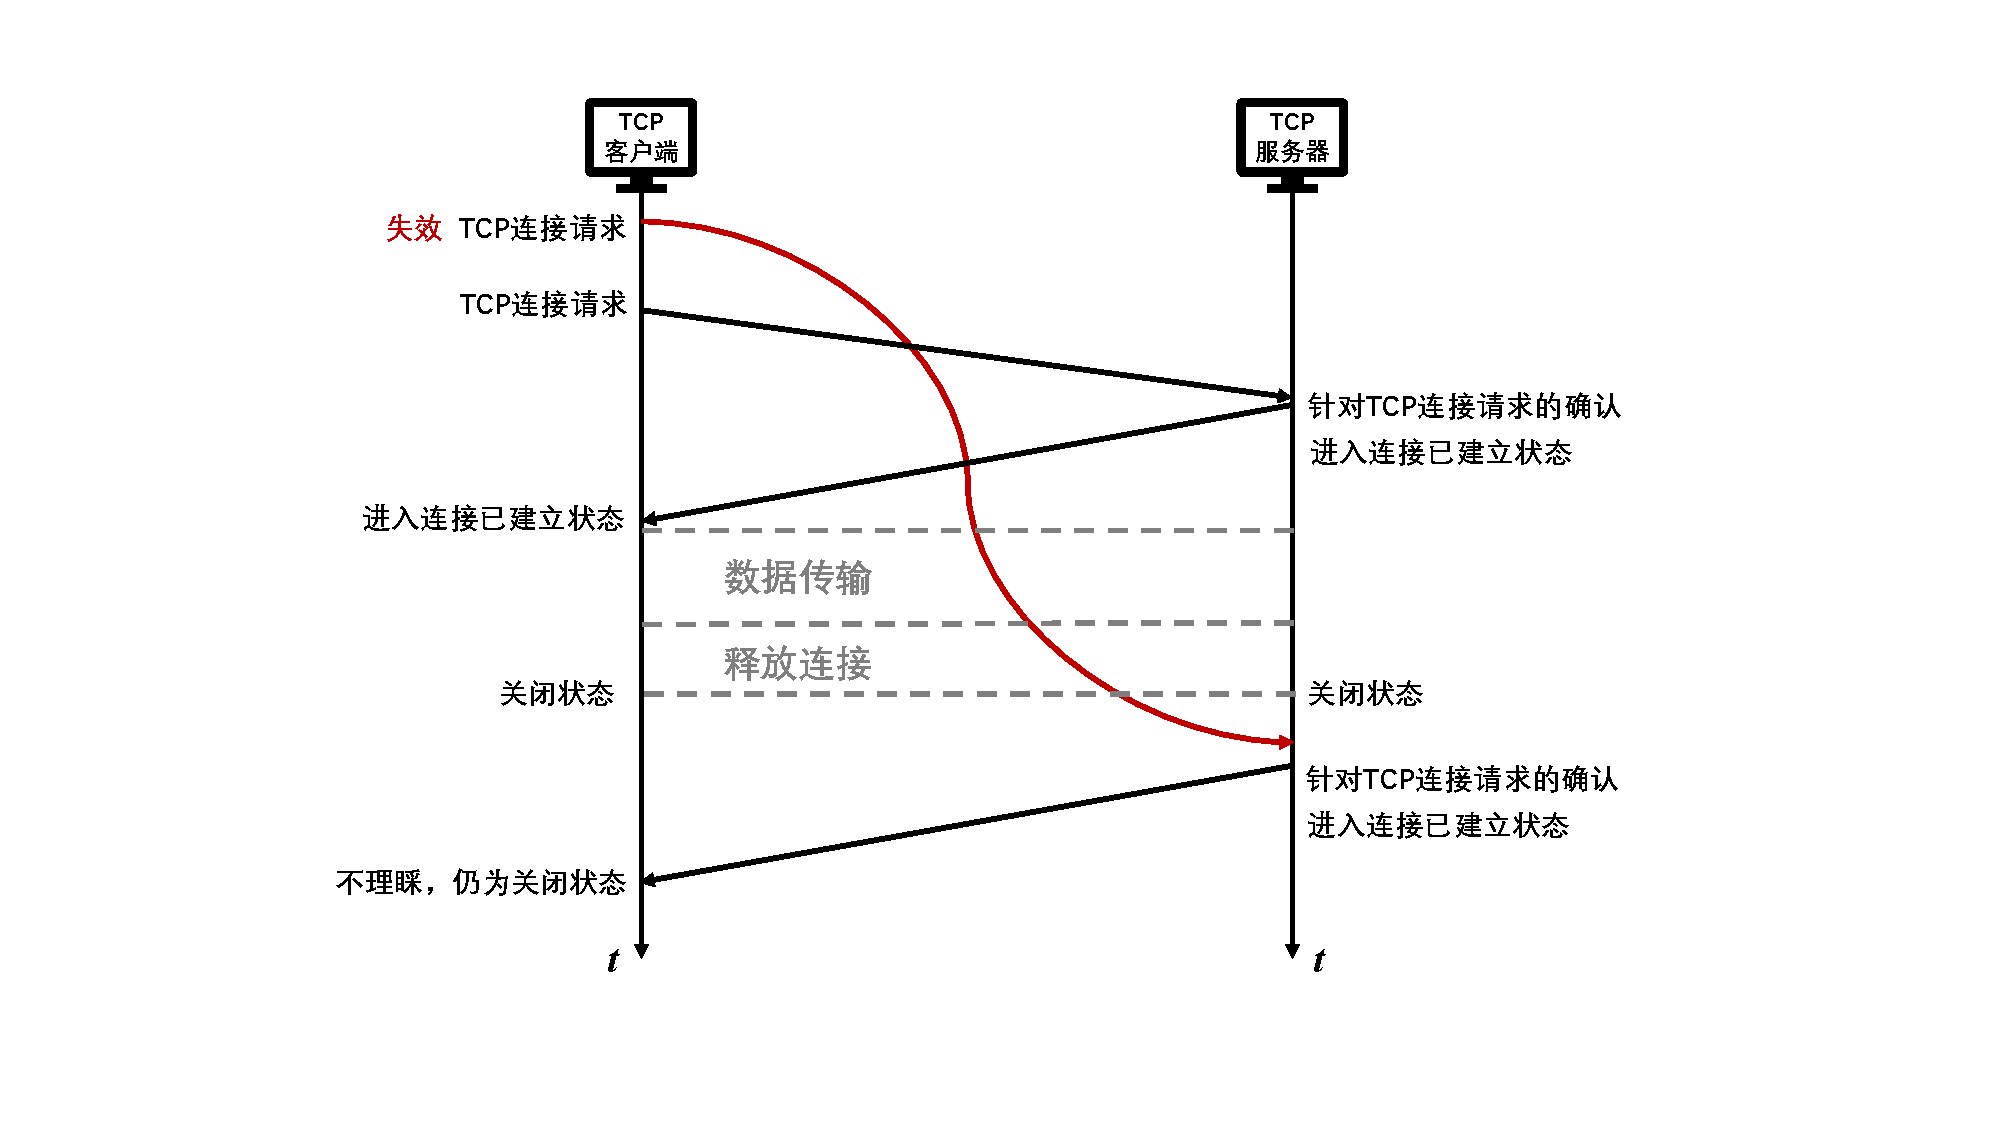
\includegraphics[width=0.65\textwidth]{img/5.8.1}
	\end{figure}

	\subsection{TCP的连接释放}

	\begin{figure}[H]
		\centering
		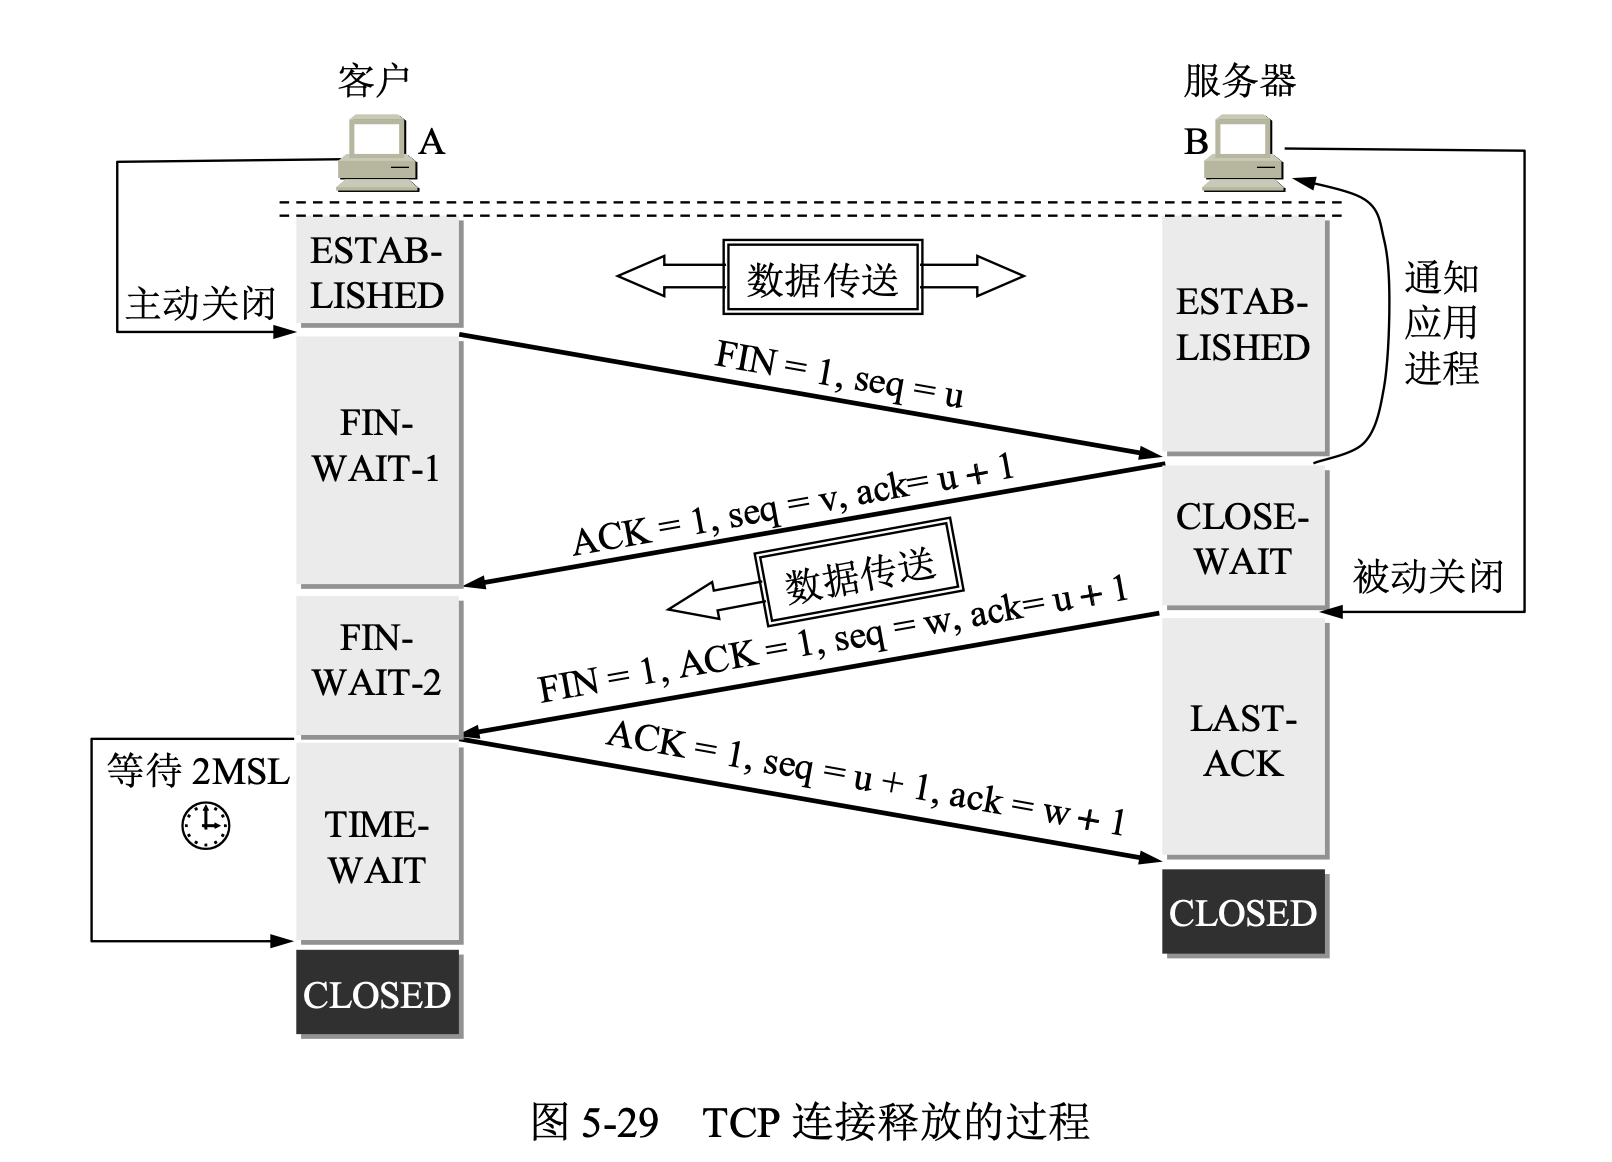
\includegraphics[width=0.7\textwidth]{img/5.29}
	\end{figure}

	数据传输结束后,通信的双方都可释放连接。现在 A 和 B 都处于 ESTABLISHED 状态

	A 的应用进程先向其 TCP 发出连接释放报文段,并停止再发送数据,主动关闭 TCP连接。A把连接释放报文段首部的终止控制位 FIN 置1,其序号 seq = $u$,它等于前面已传送过的数据的最后一个字节的序号加 1。这时 A 进入 FIN-WAIT-1(终止等待 1)状态,等待 B 的确认。请注意,TCP 规定,FIN 报文段即使不携带数据,它也消耗掉一个序号

	B 收到连接释放报文段后即发出确认,确认号是 ack = $u + 1$,而这个报文段自己的序号是 $v$,等于 B 前面已传送过的数据的最后一个字节的序号加 1。然后 B 就进入 CLOSE- WAIT(关闭等待)状态。

	TCP 服务器进程这时应通知高层应用进程,因而从 A 到 B 这个方向的连接就释放了,这时的 TCP 连接处于半关闭(half-close)状态,即 A 已经没有数据要发送了,但 B 若发送数据,A 仍要接收。也就是说,从 B 到 A 这个方向的连接并未关闭,这个状态可能会持续一段时间

	A 收到来自 B 的确认后,就进入 FIN-WAIT-2(终止等待 2)状态,等待 B 发出的连接释放报文段

	若 B 已经没有要向 A 发送的数据,其应用进程就通知 TCP 释放连接。这时 B 发出的连接释放报文段必须使 FIN = 1。现假定 B 的序号为 $w$ (在半关闭状态B可能又发送了一些数据)。B还必须重复上次已发送过的确认号 ack = $u + 1$。这时 B 就进入LAST-ACK(最后确认)状态,等待 A 的确认

	A 在收到 B 的连接释放报文段后,必须对此发出确认。在确认报文段中把 ACK 置 1,确认号 ack = $w + 1$,而自己的序号是 seq = $u + 1$,然后进入到 TIME-WAIT(时间等待)状态

	现在 TCP 连接还没有释放掉。必须经过时间等待计时器(TIME-WAIT timer)设置的时间 2MSL \footnote{时间 MSL 叫做最长报文段寿命(Maximum Segment Lifetime),RFC 793 建议设为 2 分钟。但这完全是从工程上来考虑的,对于现在的网络,MSL = 2 分钟可能太长了一些。因此 TCP 允许不同的实现可根据具体情况使用更小的 MSL 值}
	后,A 才进入到 CLOSED 状态

	B 只要收到了 A 发出的确认,就进入 CLOSED 状态

	A 在 TIME-WAIT 状态必须等待 2MSL 时间的原因:
	\begin{itemize}
		\item 防止下图所示情况的出现
		\begin{figure}[H]
			\centering
			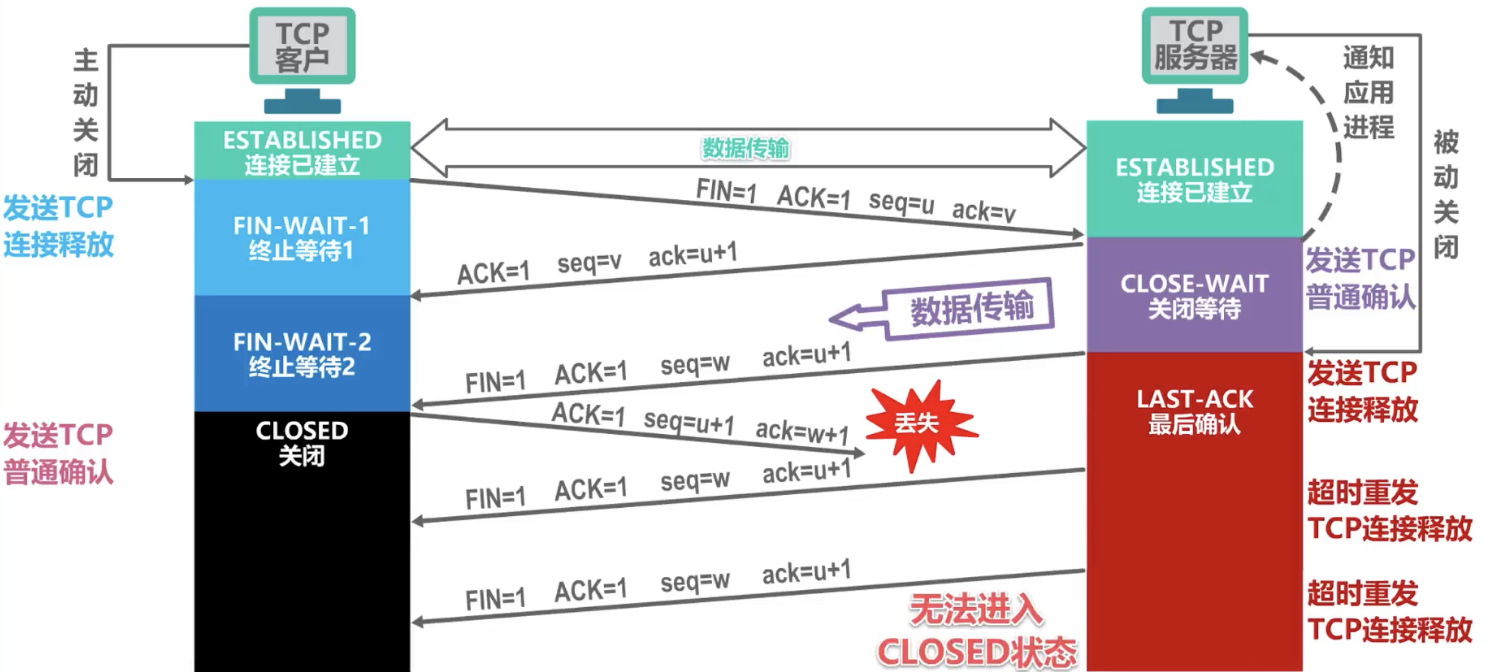
\includegraphics[width=0.75\textwidth]{img/5.8.2}
		\end{figure}
		\item 防止“已失效的连接请求报文段”出现在本连接中。A 在发送完最后一个 ACK 报文段后,再经过时间 2MSL,就可以使本连接持续的时间内所产生的所有报文段都从网络中消失。这样就可以使下一个新的连接中不会出现旧的连接请求报文段
		\begin{figure}[H]
			\centering
			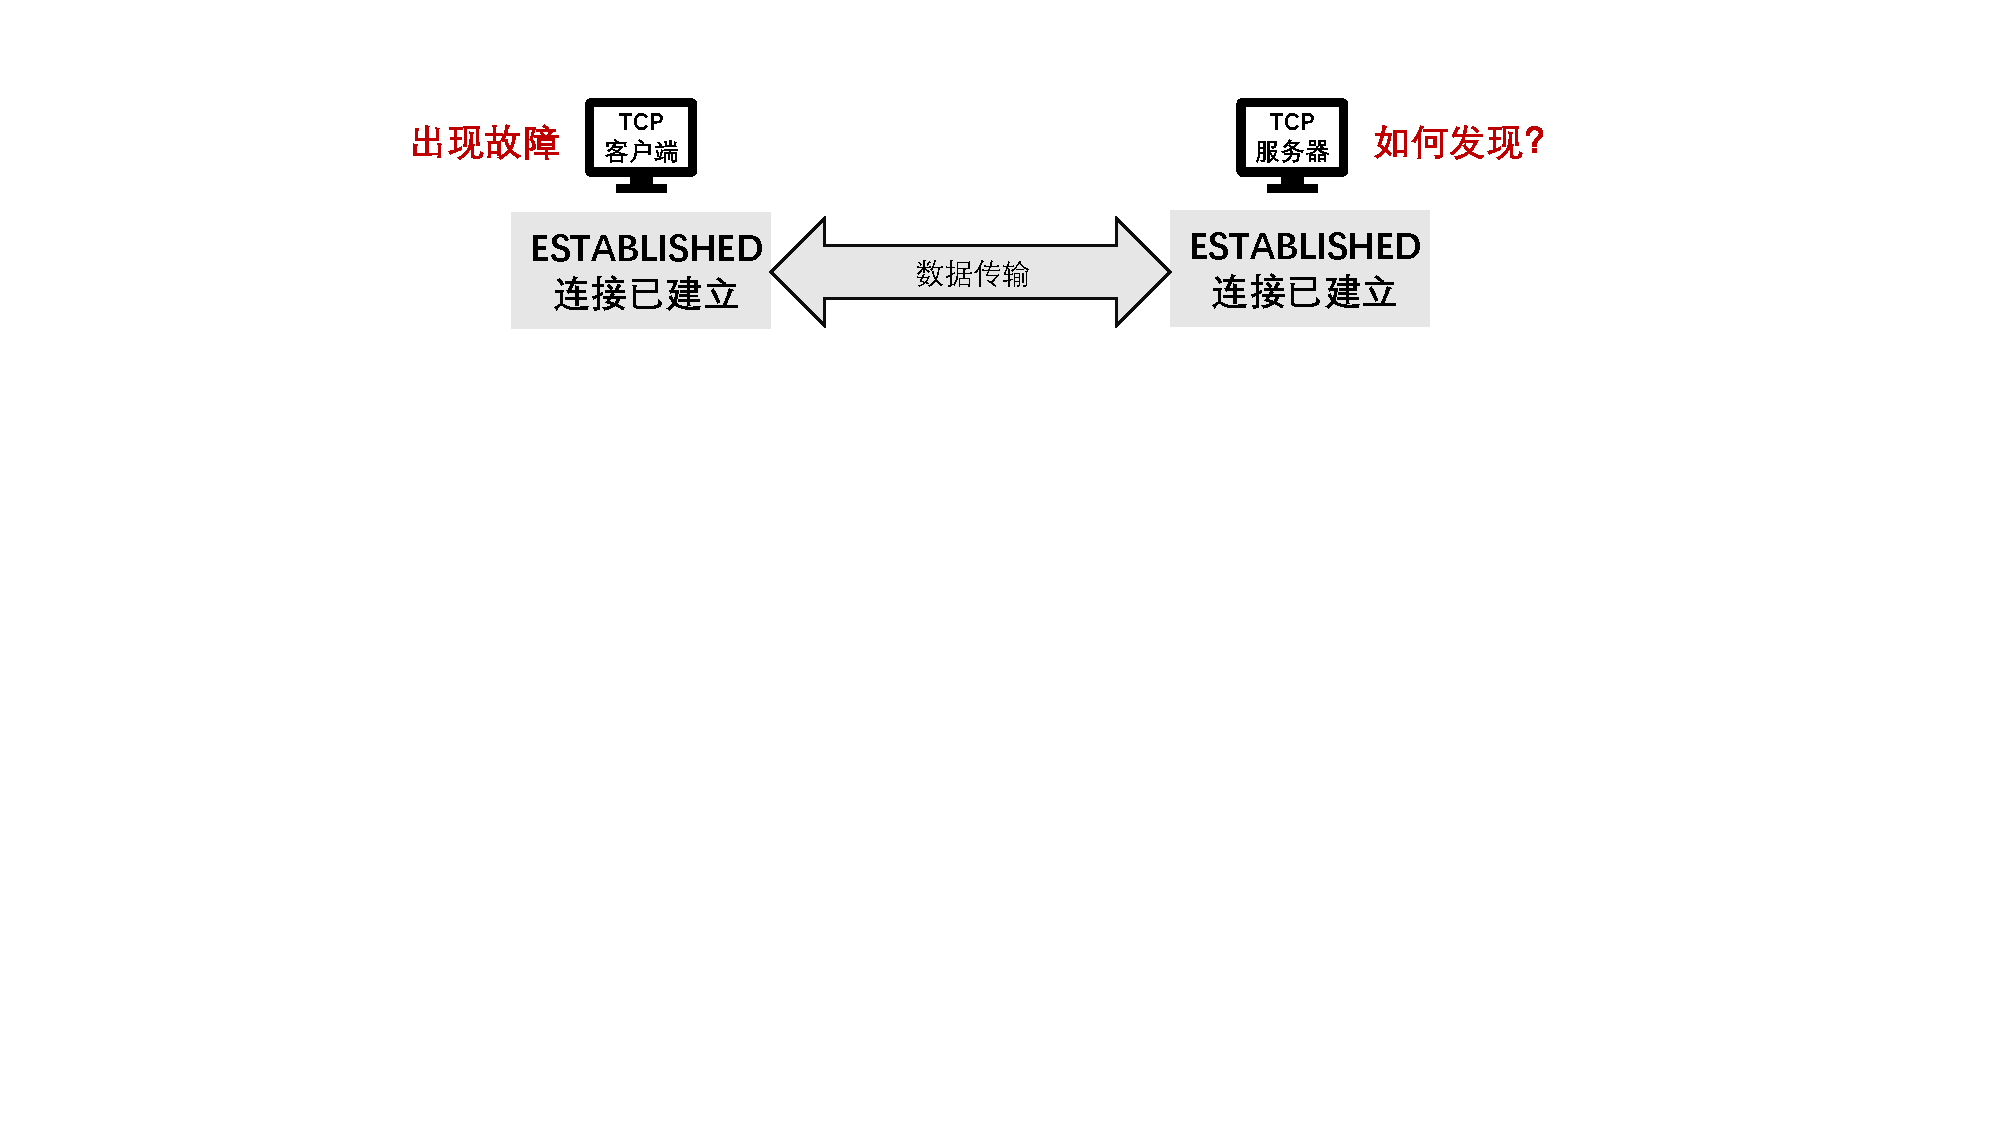
\includegraphics[width=0.45\textwidth]{img/5.8.2.2}
		\end{figure}
		\item TCP 服务器进程每收到一次 TCP 客户进程的数据,就重新设置并启动保活计时器(2小时定时)
		\item 若保活计时器定时周期内未收到 TCP 客户进程发来的数据,则当保活计时器到时后,TCP 服务器进程就向 TCP 客户进程发送一个探测报文段,以后则每隔 75 秒钟发送一次。若一连发送 10 个探测报文段仍无 TCP 客户进程的相应,TCP 服务器进程就认为 TCP 客户进程所在主机出了故障,接着就关闭这个连接
	\end{itemize}

	\subsection{TCP的有限状态机}
	\begin{figure}[H]
		\centering
		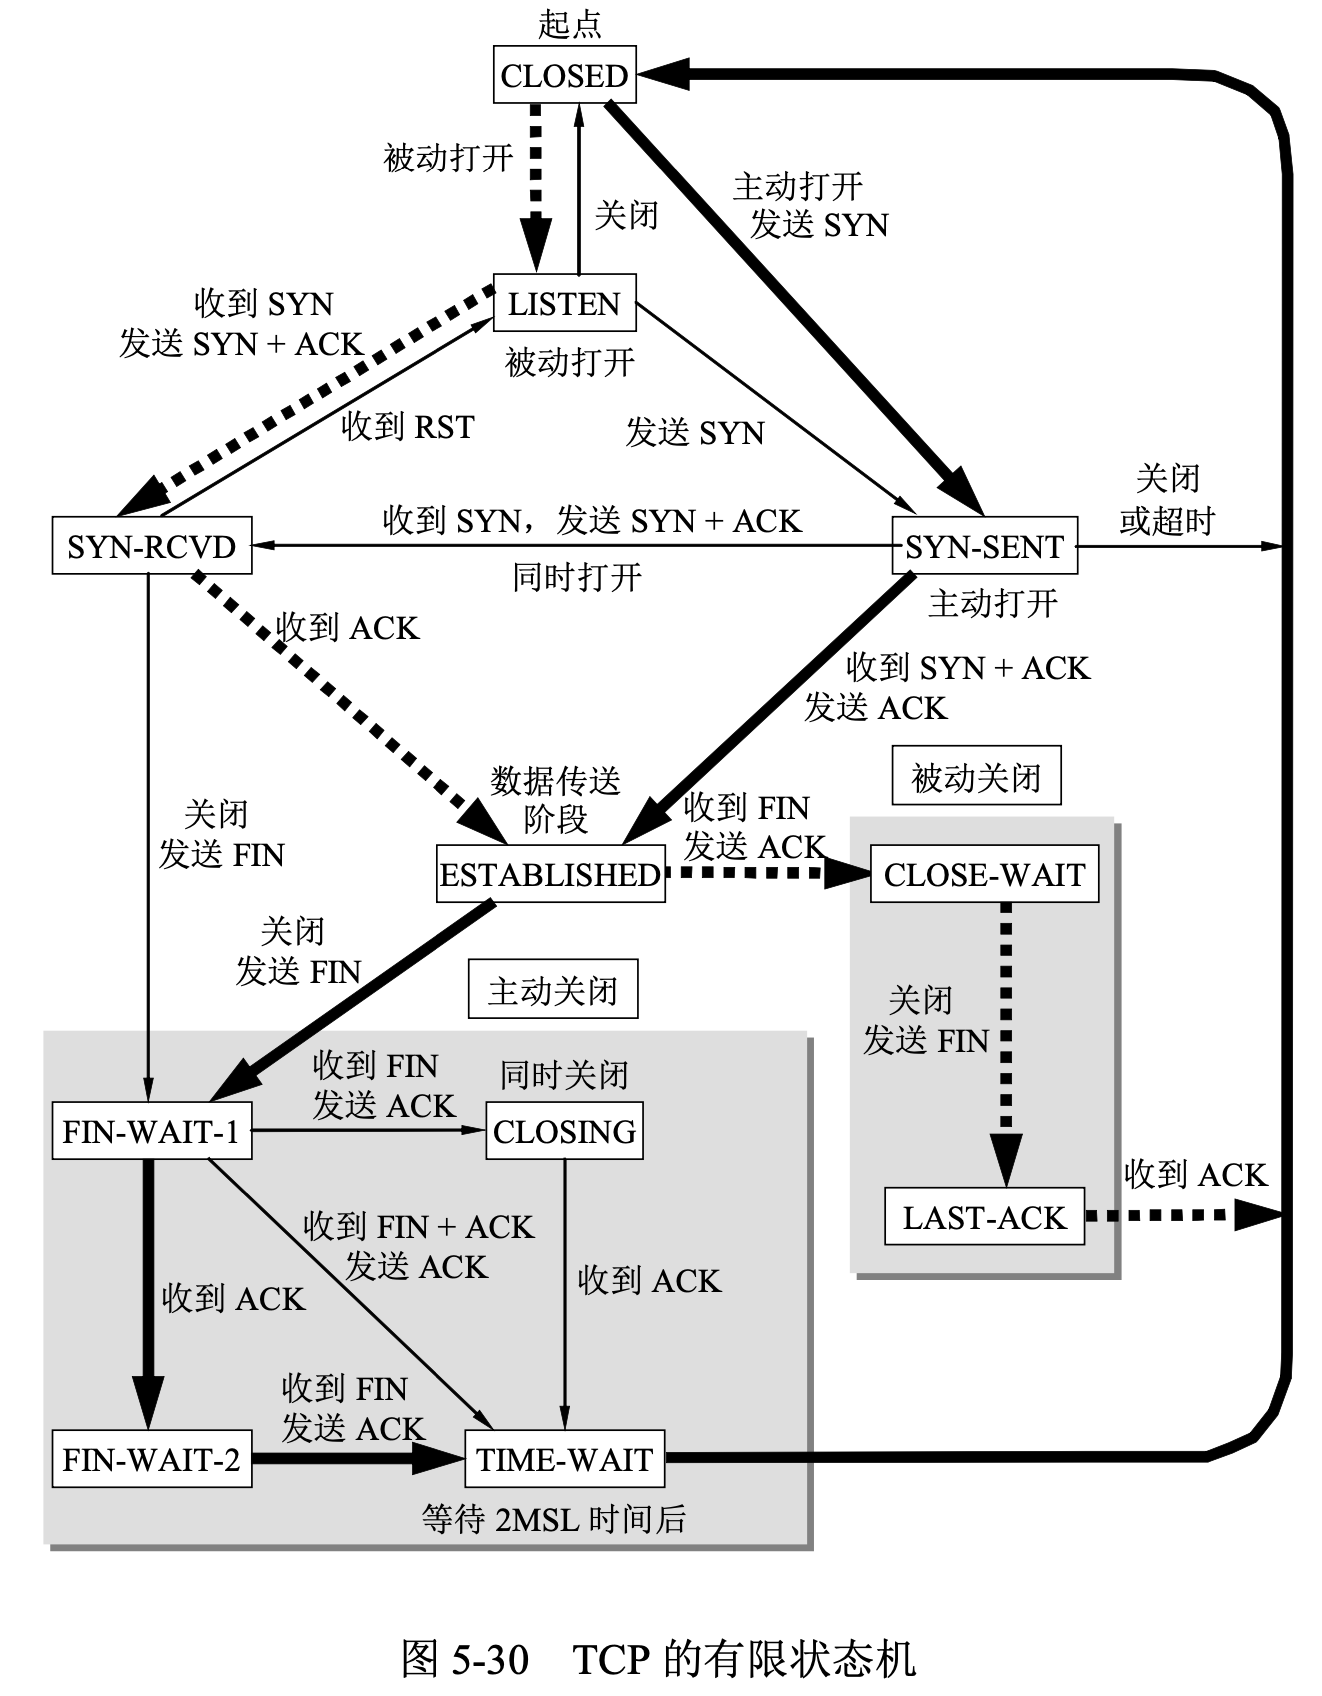
\includegraphics[width=0.8\textwidth]{img/5.30}
	\end{figure}

\end{document}


